% Options for packages loaded elsewhere
\PassOptionsToPackage{unicode}{hyperref}
\PassOptionsToPackage{hyphens}{url}
\PassOptionsToPackage{dvipsnames,svgnames,x11names}{xcolor}
%
\documentclass[
  letterpaper,
]{scrbook}

\usepackage{amsmath,amssymb}
\usepackage{iftex}
\ifPDFTeX
  \usepackage[T1]{fontenc}
  \usepackage[utf8]{inputenc}
  \usepackage{textcomp} % provide euro and other symbols
\else % if luatex or xetex
  \usepackage{unicode-math}
  \defaultfontfeatures{Scale=MatchLowercase}
  \defaultfontfeatures[\rmfamily]{Ligatures=TeX,Scale=1}
\fi
\usepackage[]{kpfonts}
\ifPDFTeX\else  
    % xetex/luatex font selection
  \setmonofont[]{FiraMono}
\fi
% Use upquote if available, for straight quotes in verbatim environments
\IfFileExists{upquote.sty}{\usepackage{upquote}}{}
\IfFileExists{microtype.sty}{% use microtype if available
  \usepackage[]{microtype}
  \UseMicrotypeSet[protrusion]{basicmath} % disable protrusion for tt fonts
}{}
\makeatletter
\@ifundefined{KOMAClassName}{% if non-KOMA class
  \IfFileExists{parskip.sty}{%
    \usepackage{parskip}
  }{% else
    \setlength{\parindent}{0pt}
    \setlength{\parskip}{6pt plus 2pt minus 1pt}}
}{% if KOMA class
  \KOMAoptions{parskip=half}}
\makeatother
\usepackage{xcolor}
\setlength{\emergencystretch}{3em} % prevent overfull lines
\setcounter{secnumdepth}{5}
% Make \paragraph and \subparagraph free-standing
\ifx\paragraph\undefined\else
  \let\oldparagraph\paragraph
  \renewcommand{\paragraph}[1]{\oldparagraph{#1}\mbox{}}
\fi
\ifx\subparagraph\undefined\else
  \let\oldsubparagraph\subparagraph
  \renewcommand{\subparagraph}[1]{\oldsubparagraph{#1}\mbox{}}
\fi

\usepackage{color}
\usepackage{fancyvrb}
\newcommand{\VerbBar}{|}
\newcommand{\VERB}{\Verb[commandchars=\\\{\}]}
\DefineVerbatimEnvironment{Highlighting}{Verbatim}{commandchars=\\\{\}}
% Add ',fontsize=\small' for more characters per line
\usepackage{framed}
\definecolor{shadecolor}{RGB}{241,243,245}
\newenvironment{Shaded}{\begin{snugshade}}{\end{snugshade}}
\newcommand{\AlertTok}[1]{\textcolor[rgb]{0.68,0.00,0.00}{#1}}
\newcommand{\AnnotationTok}[1]{\textcolor[rgb]{0.37,0.37,0.37}{#1}}
\newcommand{\AttributeTok}[1]{\textcolor[rgb]{0.40,0.45,0.13}{#1}}
\newcommand{\BaseNTok}[1]{\textcolor[rgb]{0.68,0.00,0.00}{#1}}
\newcommand{\BuiltInTok}[1]{\textcolor[rgb]{0.00,0.23,0.31}{#1}}
\newcommand{\CharTok}[1]{\textcolor[rgb]{0.13,0.47,0.30}{#1}}
\newcommand{\CommentTok}[1]{\textcolor[rgb]{0.37,0.37,0.37}{#1}}
\newcommand{\CommentVarTok}[1]{\textcolor[rgb]{0.37,0.37,0.37}{\textit{#1}}}
\newcommand{\ConstantTok}[1]{\textcolor[rgb]{0.56,0.35,0.01}{#1}}
\newcommand{\ControlFlowTok}[1]{\textcolor[rgb]{0.00,0.23,0.31}{\textbf{#1}}}
\newcommand{\DataTypeTok}[1]{\textcolor[rgb]{0.68,0.00,0.00}{#1}}
\newcommand{\DecValTok}[1]{\textcolor[rgb]{0.68,0.00,0.00}{#1}}
\newcommand{\DocumentationTok}[1]{\textcolor[rgb]{0.37,0.37,0.37}{\textit{#1}}}
\newcommand{\ErrorTok}[1]{\textcolor[rgb]{0.68,0.00,0.00}{#1}}
\newcommand{\ExtensionTok}[1]{\textcolor[rgb]{0.00,0.23,0.31}{#1}}
\newcommand{\FloatTok}[1]{\textcolor[rgb]{0.68,0.00,0.00}{#1}}
\newcommand{\FunctionTok}[1]{\textcolor[rgb]{0.28,0.35,0.67}{#1}}
\newcommand{\ImportTok}[1]{\textcolor[rgb]{0.00,0.46,0.62}{#1}}
\newcommand{\InformationTok}[1]{\textcolor[rgb]{0.37,0.37,0.37}{#1}}
\newcommand{\KeywordTok}[1]{\textcolor[rgb]{0.00,0.23,0.31}{\textbf{#1}}}
\newcommand{\NormalTok}[1]{\textcolor[rgb]{0.00,0.23,0.31}{#1}}
\newcommand{\OperatorTok}[1]{\textcolor[rgb]{0.37,0.37,0.37}{#1}}
\newcommand{\OtherTok}[1]{\textcolor[rgb]{0.00,0.23,0.31}{#1}}
\newcommand{\PreprocessorTok}[1]{\textcolor[rgb]{0.68,0.00,0.00}{#1}}
\newcommand{\RegionMarkerTok}[1]{\textcolor[rgb]{0.00,0.23,0.31}{#1}}
\newcommand{\SpecialCharTok}[1]{\textcolor[rgb]{0.37,0.37,0.37}{#1}}
\newcommand{\SpecialStringTok}[1]{\textcolor[rgb]{0.13,0.47,0.30}{#1}}
\newcommand{\StringTok}[1]{\textcolor[rgb]{0.13,0.47,0.30}{#1}}
\newcommand{\VariableTok}[1]{\textcolor[rgb]{0.07,0.07,0.07}{#1}}
\newcommand{\VerbatimStringTok}[1]{\textcolor[rgb]{0.13,0.47,0.30}{#1}}
\newcommand{\WarningTok}[1]{\textcolor[rgb]{0.37,0.37,0.37}{\textit{#1}}}

\providecommand{\tightlist}{%
  \setlength{\itemsep}{0pt}\setlength{\parskip}{0pt}}\usepackage{longtable,booktabs,array}
\usepackage{calc} % for calculating minipage widths
% Correct order of tables after \paragraph or \subparagraph
\usepackage{etoolbox}
\makeatletter
\patchcmd\longtable{\par}{\if@noskipsec\mbox{}\fi\par}{}{}
\makeatother
% Allow footnotes in longtable head/foot
\IfFileExists{footnotehyper.sty}{\usepackage{footnotehyper}}{\usepackage{footnote}}
\makesavenoteenv{longtable}
\usepackage{graphicx}
\makeatletter
\def\maxwidth{\ifdim\Gin@nat@width>\linewidth\linewidth\else\Gin@nat@width\fi}
\def\maxheight{\ifdim\Gin@nat@height>\textheight\textheight\else\Gin@nat@height\fi}
\makeatother
% Scale images if necessary, so that they will not overflow the page
% margins by default, and it is still possible to overwrite the defaults
% using explicit options in \includegraphics[width, height, ...]{}
\setkeys{Gin}{width=\maxwidth,height=\maxheight,keepaspectratio}
% Set default figure placement to htbp
\makeatletter
\def\fps@figure{htbp}
\makeatother

% using text input is not working
% _quarto.yml

\usepackage{hyperref}
\usepackage{fancyvrb,newverbs,xcolor}
\usepackage{FiraMono} 
\usepackage{tikz}
\usepackage{xcolor}
\usepackage{soul}
%\usepackage[margin=0.5in]{geometry}
%\usepackage{afterpage}

\usepackage{geometry}
 \geometry{
 letterpaper,
bottom=0.8in,
top=0.8in,
left=0.8in,
right=0.8in,
includefoot
 }

%fontsize=9pt
% \geometry{
% paperwidth=6in,
% paperheight=9in,
% bottom=0.8in,
% top=0.8in,
% left=0.8in,
% right=0.8in
% }

%\setlength{\parskip}{0pt}
%
%\usepackage[compact]{titlesec}
%\titlespacing{\section}{0pt}{2ex}{1ex}
%\titlespacing{\subsection}{0pt}{1ex}{0ex}
%\titlespacing{\subsubsection}{0pt}{0.5ex}{0ex}
\makeatletter
\@ifpackageloaded{tcolorbox}{}{\usepackage[skins,breakable]{tcolorbox}}
\@ifpackageloaded{fontawesome5}{}{\usepackage{fontawesome5}}
\definecolor{quarto-callout-color}{HTML}{909090}
\definecolor{quarto-callout-note-color}{HTML}{0758E5}
\definecolor{quarto-callout-important-color}{HTML}{CC1914}
\definecolor{quarto-callout-warning-color}{HTML}{EB9113}
\definecolor{quarto-callout-tip-color}{HTML}{00A047}
\definecolor{quarto-callout-caution-color}{HTML}{FC5300}
\definecolor{quarto-callout-color-frame}{HTML}{acacac}
\definecolor{quarto-callout-note-color-frame}{HTML}{4582ec}
\definecolor{quarto-callout-important-color-frame}{HTML}{d9534f}
\definecolor{quarto-callout-warning-color-frame}{HTML}{f0ad4e}
\definecolor{quarto-callout-tip-color-frame}{HTML}{02b875}
\definecolor{quarto-callout-caution-color-frame}{HTML}{fd7e14}
\makeatother
\makeatletter
\@ifpackageloaded{bookmark}{}{\usepackage{bookmark}}
\makeatother
\makeatletter
\@ifpackageloaded{caption}{}{\usepackage{caption}}
\AtBeginDocument{%
\ifdefined\contentsname
  \renewcommand*\contentsname{Table of contents}
\else
  \newcommand\contentsname{Table of contents}
\fi
\ifdefined\listfigurename
  \renewcommand*\listfigurename{List of Figures}
\else
  \newcommand\listfigurename{List of Figures}
\fi
\ifdefined\listtablename
  \renewcommand*\listtablename{List of Tables}
\else
  \newcommand\listtablename{List of Tables}
\fi
\ifdefined\figurename
  \renewcommand*\figurename{Figure}
\else
  \newcommand\figurename{Figure}
\fi
\ifdefined\tablename
  \renewcommand*\tablename{Table}
\else
  \newcommand\tablename{Table}
\fi
}
\@ifpackageloaded{float}{}{\usepackage{float}}
\floatstyle{ruled}
\@ifundefined{c@chapter}{\newfloat{codelisting}{h}{lop}}{\newfloat{codelisting}{h}{lop}[chapter]}
\floatname{codelisting}{Listing}
\newcommand*\listoflistings{\listof{codelisting}{List of Listings}}
\makeatother
\makeatletter
\makeatother
\makeatletter
\@ifpackageloaded{caption}{}{\usepackage{caption}}
\@ifpackageloaded{subcaption}{}{\usepackage{subcaption}}
\makeatother
\makeatletter
\@ifpackageloaded{tcolorbox}{}{\usepackage[skins,breakable]{tcolorbox}}
\makeatother
\makeatletter
\@ifundefined{shadecolor}{\definecolor{shadecolor}{rgb}{.97, .97, .97}}{}
\makeatother
\makeatletter
\@ifundefined{codebgcolor}{\definecolor{codebgcolor}{HTML}{D3D3D3}}{}
\makeatother
\makeatletter
\ifdefined\Shaded\renewenvironment{Shaded}{\begin{tcolorbox}[colback={codebgcolor}, breakable, frame hidden, boxrule=0pt, sharp corners, enhanced]}{\end{tcolorbox}}\fi
\makeatother
\ifLuaTeX
  \usepackage{selnolig}  % disable illegal ligatures
\fi
\usepackage{bookmark}

\IfFileExists{xurl.sty}{\usepackage{xurl}}{} % add URL line breaks if available
\urlstyle{same} % disable monospaced font for URLs
\hypersetup{
  pdftitle={Data Science for Crime Analysis with Python},
  pdfauthor={Andrew P. Wheeler},
  colorlinks=true,
  linkcolor={Maroon},
  filecolor={Maroon},
  citecolor={Blue},
  urlcolor={Blue},
  pdfcreator={LaTeX via pandoc}}

\title{Data Science for Crime Analysis with Python}
\author{Andrew P. Wheeler}
\date{2025-10-07}

\begin{document}
\frontmatter
\maketitle

Data Science for Crime Analysis with Python

\copyright Andrew P. Wheeler 2024

ISBN 979-8-9903770-0-4 (ebook), ISBN 979-8-9903770-1-1 (paperback)

All rights reserved. No part of this publication may be produced or transmitted in any
form or by any means without prior written permission, with the exception of small excerpts for review. 
For permission contact Andrew P. Wheeler at andrew.wheeler@crimede-coder.com.

You can see my other work at \url{https://crimede-coder.com/}

\begin{tikzpicture}[scale=0.05]
\node[xshift=-1.5in,yshift=-1.5in]{
\includegraphics{chap_images/WLineRec.PNG}};
\end{tikzpicture}

% macros file to define verbatim environment
% which is the output of code samples
% https://tex.stackexchange.com/a/141128/8217

%\usepackage{fancyvrb,newverbs,xcolor}
%\usepackage{soul}

%\definecolor{cverbbg}{gray}{0.93}
\definecolor{cverbbg}{HTML}{ADD8E6}

\renewenvironment{verbatim}
 {\SaveVerbatim{cverb}}
 {\endSaveVerbatim
  \flushleft\fboxrule=0pt\fboxsep=.5em
  \colorbox{cverbbg}{%
    \makebox[\dimexpr\linewidth-2\fboxsep][l]{\BUseVerbatim{cverb}}%
  }
  \endflushleft
}

% https://gist.github.com/wusunlab/9c85fcb7472308a474e7c3fb443639ee
\definecolor{inlineBG}{HTML}{D3D3D3}
\sethlcolor{inlineBG}
\let\OldTexttt\texttt
\renewcommand{\texttt}[1]{\sethlcolor{inlineBG}{\ttfamily\hl{\mbox{#1}}}}

% https://tex.stackexchange.com/a/86702/8217
% to draw tikz in background

%https://tex.stackexchange.com/questions/70547/how-can-i-renew-includegraphics-to-always-use-shadowbox

\raggedbottom

\renewcommand*\contentsname{Table of Contents}
{
\hypersetup{linkcolor=}
\setcounter{tocdepth}{1}
\tableofcontents
}
\mainmatter
\bookmarksetup{startatroot}

\chapter*{Preface}\label{preface}
\addcontentsline{toc}{chapter}{Preface}

\markboth{Preface}{Preface}

Python is an open-source, free, computer programming language. It allows
you to write simple (or complex) programs, to allow your computer to
accomplish tasks. For a brief example, here is a python code snippet
that tells you the difference in the number of days between two dates.
The lines that start with \texttt{\#} are comments in python, the other
lines perform different operations in python code. The text in the grey
portion below is the python code, and the blue section text is the
output of the program.

\begin{Shaded}
\begin{Highlighting}[]
\CommentTok{\# importing library to calculate times}
\ImportTok{from}\NormalTok{ datetime }\ImportTok{import}\NormalTok{ datetime}

\CommentTok{\# creating two datetime objects}
\NormalTok{begin }\OperatorTok{=}\NormalTok{ datetime(}\DecValTok{2022}\NormalTok{,}\DecValTok{1}\NormalTok{,}\DecValTok{16}\NormalTok{)}
\NormalTok{end }\OperatorTok{=}\NormalTok{ datetime(}\DecValTok{2023}\NormalTok{,}\DecValTok{1}\NormalTok{,}\DecValTok{16}\NormalTok{)}

\CommentTok{\# calculating the difference}
\NormalTok{dif }\OperatorTok{=}\NormalTok{ end }\OperatorTok{{-}}\NormalTok{ begin}

\CommentTok{\# printing the result}
\BuiltInTok{print}\NormalTok{(dif.days)}
\end{Highlighting}
\end{Shaded}

\begin{verbatim}
365
\end{verbatim}

So this is a trivial program -- you could figure out the number of days
between the two dates using various tools. The power of being able to
program in python is that you can write computer code to do (close to)
any computation you want. A common example for a crime analyst may be
querying a database and creating a table of crime counts year-to-date
this year vs last. You can then run the code at will, and it will update
the year-to-date stats on whatever frequency you want. Such a report in
practice will just be chaining together short code examples like above
into more complicated series of operations.

\section*{Who is this book for?}\label{who-is-this-book-for}
\addcontentsline{toc}{section}{Who is this book for?}

\markright{Who is this book for?}

This book is aimed at individuals with no (or beginner) background in
programming, but who are interested in using code to conduct
quantitative analysis and automate tasks. The main intended audience of
the book are crime analysts, but any individual looking to get started
in coding and data analysis should find the content of the book useful.
Besides crime analysts, those wishing to advance their career in a data
science role or pursue graduate level research (who have a background in
criminal justice), will find the book and its examples useful.

There are many current resources on using python on the internet -- one
can use a search engine to find various entirely free resources online.
I commonly blog on technical computing at
\href{https://andrewpwheeler.com/}{andrewpwheeler.com}, which is free
for anyone to read. These free resources are often haphazard though, and
are very difficult for newcomers to understand and get started. Things
like ``How do I run a simple python script'' or ``How do I install a
python library'' are not typical topics covered in even introductory
python materials online. This book is intended to make a singular
resource for individuals in crime analysis to get started.

I intend this book to not only introduce code examples in python, but to
also describe other necessary steps for beginners, such as setting up
python environments and automating tasks using shell scripts. Don't
worry if you do not understand what those are at the moment -- they will
be explained! I even spend time describing a typical project structure
that is fairly standard across more professional software development.
These are things not related to coding directly, but are necessary to be
able to get started using python and use it effectively.

So this book fills a niche -- an introduction to doing tasks in python
of relevance to crime analysts. The book subsequently contains:

\begin{itemize}
\tightlist
\item
  installing and creating python environments
\item
  an introduction to python programming
\item
  working with tabular data using scientific libraries
\item
  using SQL to query databases
\item
  automating report creation and creating high quality tables and graphs
\end{itemize}

These are the necessary ingredients, both in terms of coding and doing
more realistic projects, that allow one to become more productive in
their regular tasks using python.

\section*{What this book is not}\label{what-this-book-is-not}
\addcontentsline{toc}{section}{What this book is not}

\markright{What this book is not}

When approaching learning to code and data analysis, many books include
\emph{both} at the same time. This is often a mistake, as it can greatly
increase the burden on those wishing to learn the material. This book
\emph{is not} meant as an introduction to crime analysis as a topic in
general. For those who wish to learn basic statistics and analyses that
crime analysts conduct, I would suggest to check out the course
materials on my personal website, as well as the materials from the
International Association of Crime Analysts (IACA). If demand is
sufficient, I may create future books to cover intro statistics for
crime analysts more thoroughly, so let me know if that is something you
are interested in!

This book is aimed to get you started writing code and applying it to
real tasks crime analysts need to conduct. I use realistic examples that
a crime analyst may be interested in conducting, such as sending
automated emails, making year-to-date tables, and creating line charts.
But I do not discuss in detail things like the Poisson distribution for
analyzing crime rates or why hotspot analyses is important.

While the material is definitely relevant to \emph{everyone} who needs
to conduct data analysis using python, I hope to use more realistic
crime analysis examples to better illustrate the utility of using python
to conduct analyses in your day-to-day tasks as a crime analyst.

\section*{Why learn to code?}\label{why-learn-to-code}
\addcontentsline{toc}{section}{Why learn to code?}

\markright{Why learn to code?}

Crime analysts do much of their quantitative work in spreadsheets
(e.g.~Excel), and then a smaller number use additional tools, such as
databases (e.g.~Access, SQLServer), formatted documents (Word,
Powerpoint, PDF), and GIS tools (such as ESRIs ArcMap). Why bother to
learn python? I agree that Excel can be used to do amazing things with
data, and many tasks are \emph{exchangeable} between python and one (if
not several) different tools.

The power of using programming, as opposed to tools that use a graphical
user interface (e.g.~point and click in the \emph{GUI}), are:

\begin{itemize}
\tightlist
\item
  tasks can be fully automated
\item
  tasks are fully documented
\end{itemize}

The first bullet point is an argument based on potential time savings
for automating tasks. Say it takes you 30 minutes to do a task on a
daily basis. If you take 100 hours to write python code to automate the
task entirely, you have saved yourself time within 50 days from the
automated process.

Many regular reports that crime analysts work on this time savings
argument may not be compelling though. For example, when I worked as an
analyst I had a monthly CompStat report with various graphs and maps.
Using GUI tools it maybe took me 24 hours (three working days) to
complete. Once I wrote code to automatically create the graphs, it was
under a day task. But I maybe spent over 160 hours writing code to
automate that task. It would take over a year to break even in terms of
time savings.

Many regular reports crime analysts write will look like the latter;
they will only be semi-regular, and so the time savings argument for
automating via code is not as impressive. (Code automation makes more
sense for time savings for things that need to be done more often.) Even
in those cases of semi-regular reports though, I believe writing code to
automate as much as possible is still worth it.

This is because of the second bullet point -- tasks when written in code
are by their nature fully documented. This provides the ability for an
analyst to retrospectively say things like ``this number looks weird,
how did I calculate that?'', or when a new analyst comes in and takes
over the job, you can say ``just go look at the scripts in folder X''.
Having standardized code provides a much more professional and
transparent environment, which is helpful for you as an analyst as well
as the organization as a whole.

It additionally allows you to scale your work. If you need to loan out
your time forever for a particular task, even if only a single day per
month for a particular report, you can only expand the scope of the work
you do a certain amount. Being able to automate the boring stuff is a
necessary step to free up your time to pursue other projects. It even
allows you to go on vacation, and reporting requirements can still be
fulfilled. Ultimately learning to code will likely make you more
productive when conducting ad-hoc data analysis, as well as make you
more marketable in a wider array of jobs (such as private sector data
science jobs).

\section*{Why python?}\label{why-python}
\addcontentsline{toc}{section}{Why python?}

\markright{Why python?}

The section above only describes why one would want to write code to
automate tasks, it does not detail why to use python specifically (over
say R or another statistical program). In addition to python, I have
used SPSS (a program you need to pay for), and R (another open source
statistical program) fairly extensively over my career. I have an R
package, \href{https://github.com/apwheele/ptools}{ptools}, for regular
functions of interest to crime analysts for example.

I have almost entirely migrated my personal coding to python, and do not
use these other tools very often anymore. Again, python is very
exchangeable with R for many tasks, but I prefer python at this point in
my career due to its ability to manage entire projects, not just do a
single task. In addition to this, many private sector data science
positions focus almost entirely on python (and less so on R). So I
believe in terms of professional development, especially if you have a
goal for expanding your skills to pursue private sector data science
positions, python is a better choice than R.

There are situations when paid for tools are appropriate as well.
Statistical programs like SPSS and SAS do not store their entire dataset
in memory, so can be very convenient for some large data tasks. ESRI's
GIS (\emph{Geographic Information System}) tools can be more convenient
for specific mapping tasks (such as calculating network distances or
geocoding) than many of the open source solutions. (And ESRI's tools you
can automate by using python code as well, so it is not mutually
exclusive.) But that being said, I can leverage python for nearly 100\%
of my day to day tasks. This is especially important for public sector
crime analysts, as you may not have a budget to purchase closed source
programs. Python is 100\% free and open source.

\section*{How to read this book}\label{how-to-read-this-book}
\addcontentsline{toc}{section}{How to read this book}

\markright{How to read this book}

I believe the optimal way to consume the material in this book is via a
two step process. Your level of experience with python (either some or
zero), will alter what materials you focus on and what ones you can
likely skip. For everyone, I would suggest \emph{skimming} each chapter
briefly from the start, and understanding the high level goals each
chapter is trying to teach.

This is how I personally consume technical material. You need to
understand the high level goals that any particular piece of code is
trying to accomplish before you can understand the finer technical
details. If you cannot understand the high level goals, it will be very
difficult to understand the technical details. It is also useful to
understand what is possible -- you do not need to point and click in
excel to regenerate that CompStat report every month, you can write code
to automate that (see Chapter 10).

The second part, after the skimming, is where it depends on whether you
are neophyte to python, or whether you have some background experience
in programming. For those neophytes with no experience, I would suggest
you study in detail the entry chapters 1 through 4 in the book. A large
problem in learning to run code is the ``getting started running a
simple example'' problem -- downloading a program and running commands
is challenging for those who have never done it before.

This part -- figuring out how to install python and run a simple command
can be the most challenging hurdle to get started. Part of the
challenge, as the author, is that everyone's systems is slightly
different and changing over time. Instructions to get started tend to be
idiosyncratic to your personal computer. Part of the reason I am writing
this book is that most beginner materials do not even try to discuss
this issue, and use tricks (such as using online platforms) to help
people get started.

To accomplish real tasks crime analysts need for their jobs though, you
cannot use the online platforms. Many individuals who are taught python
in university courses use said online platforms (e.g.~if you only have
experience using Jupyter notebooks or only experience with Google Collab
notebooks). You need to know how to download python and run it locally
on your personal computer to be able to use it for work related tasks.
But do not despair if you are having problems getting started! One
technique professional software engineers use is called pair-programming
-- grab a friend who knows how to run python code (which can be me, or
someone else in your network), look over their shoulder, and then have
them look over your shoulder. This will help you get started in Chapter
1.

Chapters 2 through 4 introduce basic objects (strings, numbers, lists,
dictionaries), and actions (conditional statements, looping, string
substitution). These are very boring python basics -- similar to how
learning the normal distribution is boring in your introductory stats
class, or learning algebra is boring in mathematics. They are the
necessary building blocks though for understanding how to effectively
write python code. Those with more entry level experience may feel
comfortable skimming chapters 2-4; I would suggest to examine them in a
cursory fashion at least though -- there are likely a few things you did
not know that will be introduced.

Chapter 5 is a section that even those with introductory experience
often are not exposed. Writing your own functions and understanding how
to import those functions are an important step from writing hobby code
to creating a professional environment to develop work projects over
time. Again, many individuals who have had a course in college on python
programming are not exposed to this.

Chapters 6 through 9 are oriented around showing specific examples of
working and presenting data that will be of wide interest, not only to
those in crime analysis but those in any data oriented role. Chapter 6
shows the two main libraries to work with tabular data -- \texttt{numpy}
and \texttt{pandas}. Understanding the pandas library in particular is
an important skill for those using python to conduct data analysis.

Chapter 7 shows how to use python to generate SQL queries. For those who
are not familiar with SQL, \emph{Structured Query Language}, SQL is used
to pull data from an external database and into a pandas dataframe. This
chapter I will also introduce different SQL statements, as in some
scenarios it is better to do certain data analysis tasks in the database
\emph{before} you load the data into an in-memory pandas dataframe.

Chapter 8 introduces the \texttt{matplotlib} graphing library in python.
Creating professional looking graphics is an important skill for data
analysts. Generating high quality graphs is a signal to consumers of the
quality of the work (for crime analysts these might be police officers,
command staff, or the general public). Generating such graphs via code
in python is a good way to control the look and consistency of graphs
you produce.

Chapter 9 introduces Jupyter notebooks -- notebooks offer a different
environment than the terminal to run code. Jupyter notebooks can
intermix plain text description, executable cells for code, and the
output from those code executions (e.g.~graphs and tables). This book,
under the hood, is compiled from a series of Jupyter notebooks. I
introduce Jupyter, as it is a convenient way to create standardized
reports that contain different elements of data analysis.

The final chapter 10, \emph{project organization}, discusses aspects of
project management and workflow automation -- the final necessary
components to be able to take simple projects and really leverage python
to help you do your job as a crime analyst. Now that you know how to
write code, what does a project look like? There are standard ways you
should organize your project, so when either you need to re-run the
code, or others need to, they can understand the necessary components.
This involves things like creating a README that has information to
replicate the necessary environment to run the code, having functions
documented and stored in a specific location, and a clear entry point
that runs the code in an automated fashion.

The overall contents of the book are intended to go beyond ``how to
write python code'', to giving individuals the end-to-end experience of
creating realistic projects that can help crime analysts do their job.
This involves more than just running a single script, but knowing how
professionals do things like query a database, create reusable
functions, and set up projects to automate different data analysis tasks
over time.

These not writing code portions are what is severely lacking in current
python programming how-tos, and is the main motivation to write the
book.

\section*{My background}\label{my-background}
\addcontentsline{toc}{section}{My background}

\markright{My background}

While getting my doctorate degree in criminal justice at SUNY Albany
(between 2008 and 2015), I worked in several analyst roles. First, at
the Division of Criminal Justice Services for New York state. That job
mainly involved writing standardized reports based on the New York
states criminal arrest history database. Then for several years I worked
in-house at the Troy, NY police department as their lone crime analyst.
Finally, I worked as a research analyst at the Finn Institute for Public
Safety, a non-profit who collaborated in research projects with police
departments in upstate New York.

I then was a professor of criminology for several years at the
University of Texas at Dallas, from 2016 through 2019. During that time
I wrote around 40 peer reviewed publications and collaborated on
quantitative projects with police departments across the United States.
I regularly presented this work at the IACA conference, and for a brief
period was the head of the publications committee for IACA.

Currently (since late 2019), I have worked as a data scientist (in the
private sector) for a healthcare company. My job now is to write
software, focused on using predictive models in relation to healthcare
claims data. While healthcare may seem quite different than crime
analysis, many of the problems are fundamentally the same (working with
health insurance claims is not all that different than working with
crime reports). Examples of things I have built at my current private
sector job are predictive models to identify when claims are overpaid,
or when individuals are at high risk of a follow up heart attack.

The skills to build those predictive models are no different from work I
have done forecasting crime in different areas, or identifying chronic
offenders at high risk of committing future violence. So my personal
experience as a crime analyst, a researcher, and then a private sector
data scientist are what motivated me to write this book. I want to see
some of the more advanced work in academia, as well as the software
engineering practices in the private sector, trickle down more broadly
into the crime analysis profession. An introductory book I believe is
the best method to accomplish that goal.

\section*{Feedback on the book}\label{feedback-on-the-book}
\addcontentsline{toc}{section}{Feedback on the book}

\markright{Feedback on the book}

For feedback on the contents of the book, you can send a message to me
at \url{https://crimede-coder.com/contact}. Always feel free to send me
feedback, suggest additional topics, or let me know of errors. If you
are interested in more direct services, such as in person training for
your analysts or direct consulting on projects you are working on, feel
free to email me as well. Examples of past work I have conducted for
various criminal justice agencies are program evaluation, redistricting,
automating different processes, civil litigation consulting, and
generating predictive models.

I have future plans as well to generate more advanced python content.
These include books on:

\begin{itemize}
\tightlist
\item
  more advanced programming, data, and package management
\item
  regression modeling
\item
  machine learning applications in crime analysis
\item
  GIS analysis with python
\end{itemize}

Feedback on content and letting me know what you are interested in helps
me prioritize on this future work. And more sales of this individual
book also give me motivation to write more -- so tell your friends if
you like it.

\section*{Thank you}\label{thank-you}
\addcontentsline{toc}{section}{Thank you}

\markright{Thank you}

Thanks are in order for several friends for reviewing early drafts of
the book and providing critical feedback. Renee Mitchell gave me early
feedback on drafts, and was one of the major impetuses to start this
idea and finish it. Dae-Young Kim has been diligent in giving me very
detailed feedback on each chapter, most importantly when I need to
explain the code in more detail or my narrative is not consistent with
the code examples. And I thank my wife for early feedback on the
beginning chapters writing python code. (Easily the hardest part of
coding is understanding how to run the code, not writing the code
itself. A good test to see if your documentation is sufficient is to
have someone who is \emph{not} a programmer see if they can understand.)

Thank you all for the support, and for all of those who purchased
pre-versions of the book.

This book is only possible based on various open source contributions. I
am using the Quarto engine to render this book to different environments
(PDF and EPUB), which itself uses \LaTeX~and Pandoc under the hood.
Python itself is open source, and I extensively use tools by Anaconda.
My thanks to all those individuals who help make the world go round
behind the scenes.

\bookmarksetup{startatroot}

\chapter{Setting up python}\label{setting-up-python}

\begin{tikzpicture}[overlay, remember picture]
\node[xshift=-1.5in,yshift=-1.5in] at (current page.north east) {
\includegraphics{chap_images/C01_latex.png}};
\end{tikzpicture}

First, before we can get started \emph{writing code}, we need to set up
python on your local machine. My suggestion for crime analysts is to
install the Anaconda version of python, which can be downloaded for your
machine at \url{https://www.anaconda.com/download}. I am writing this
book on Windows, but most of my advice should also extend to Mac and
Unix users (you can download Anaconda and run python on any of those
operating systems). Where it might make a difference, I will provide a
callout note. For example:

\begin{tcolorbox}[enhanced jigsaw, toprule=.15mm, rightrule=.15mm, arc=.35mm, opacityback=0, coltitle=black, bottomrule=.15mm, left=2mm, opacitybacktitle=0.6, bottomtitle=1mm, colback=white, colframe=quarto-callout-note-color-frame, colbacktitle=quarto-callout-note-color!10!white, titlerule=0mm, breakable, title={Note}, toptitle=1mm, leftrule=.75mm]

When using different paths to file locations, windows machines use
backslashes, e.g.~\texttt{C:\textbackslash{}Users\textbackslash{}andre},
whereas Mac and Unix machines use forward slashes,
\texttt{/users/andre}.

\end{tcolorbox}

Once Anaconda is installed, go ahead and open up the \emph{Anaconda
command prompt} (treat this just the same as any program you have
installed on your machine, so on Windows can navigate the programs that
pop up when clicking the Windows icon on the lower left). Once the
Anaconda command prompt is open, it should look like something below.

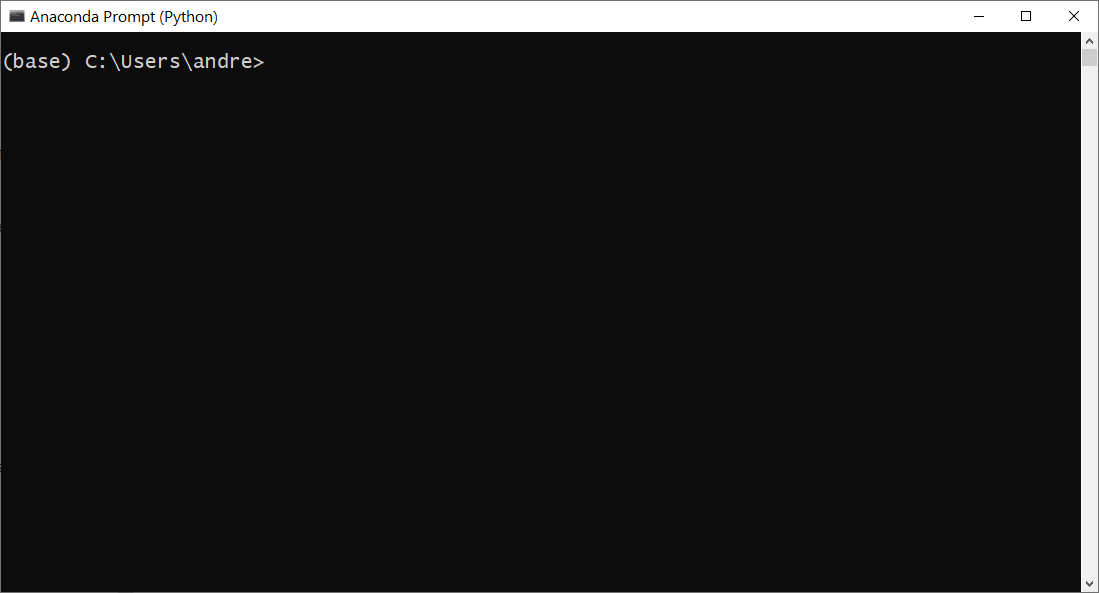
\includegraphics{screenshots/Ch01_00.PNG}

Go ahead and type \texttt{python\ -\/-version} into the command prompt,
hit enter, and see what the results are. This will tell you if you have
installed python correctly! My python version is \texttt{3.8.5}. Your
version may be different than the one I wrote this book with, but the
content I will be covering in this book it will not make a difference.

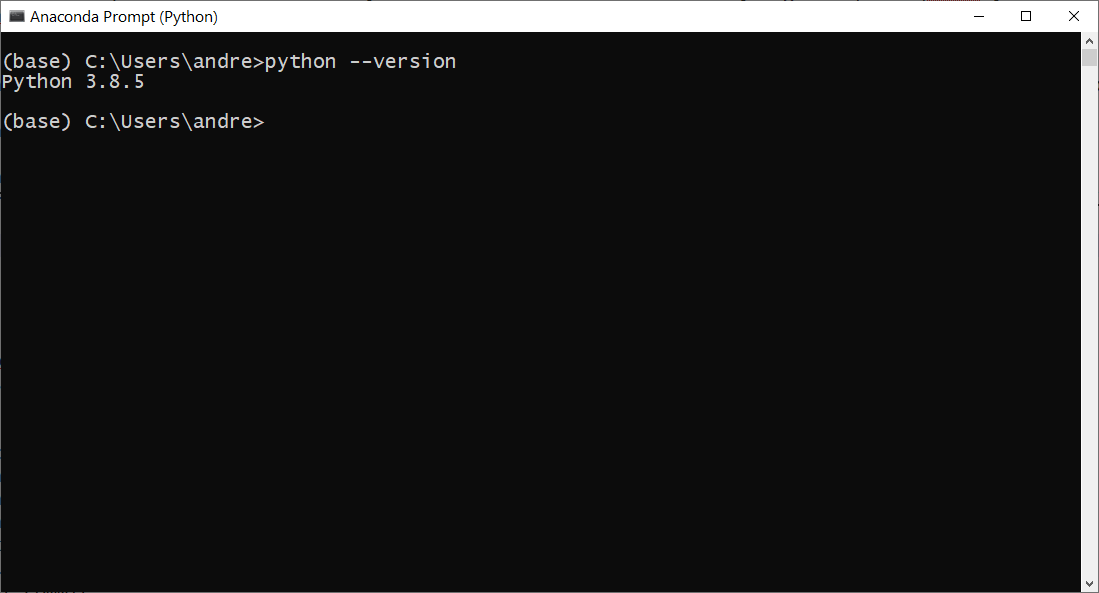
\includegraphics{screenshots/Ch01_01.PNG}

\section{Running in the REPL}\label{running-in-the-repl}

Now, we are going to run an interactive python session, sometimes people
call this the \emph{REPL}, read-eval-print-loop. Simply type
\texttt{python} in the command prompt and hit enter. You will then be
greeted with this screen, and you will be inside of a python session.

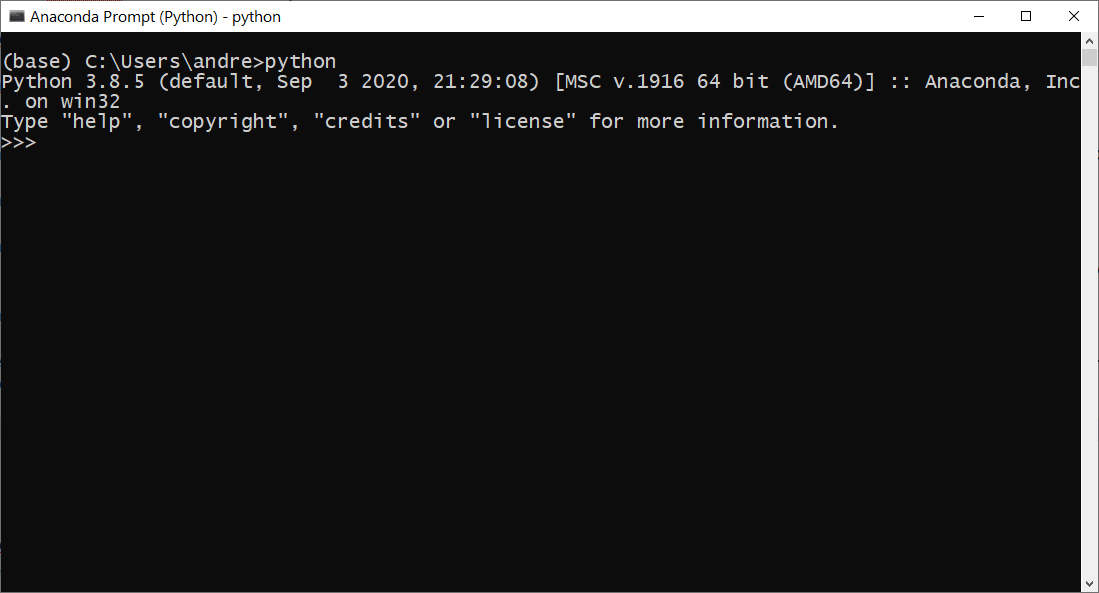
\includegraphics{screenshots/Ch01_02.PNG}

The cursor in the terminal should be located at the
\texttt{\textgreater{}\textgreater{}\textgreater{}} part of the screen.
Now at the prompt simply type \texttt{1\ +\ 2}, hit enter, and it will
output the answer:

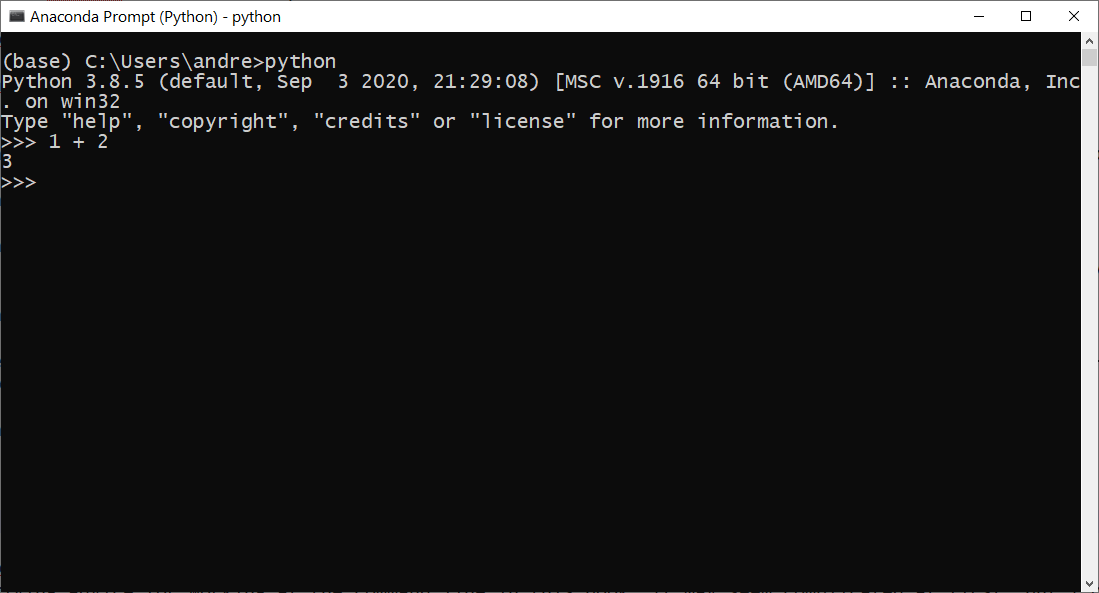
\includegraphics{screenshots/Ch01_03.PNG}

Congrats, you have now written python code.

\begin{tcolorbox}[enhanced jigsaw, toprule=.15mm, rightrule=.15mm, arc=.35mm, opacityback=0, coltitle=black, bottomrule=.15mm, left=2mm, opacitybacktitle=0.6, bottomtitle=1mm, colback=white, colframe=quarto-callout-note-color-frame, colbacktitle=quarto-callout-note-color!10!white, titlerule=0mm, breakable, title={Note}, toptitle=1mm, leftrule=.75mm]

Note the location of the cursor at the terminal at this point should be
on the \texttt{\textgreater{}\textgreater{}\textgreater{}} line. You
cannot go up to a prior line in the terminal, like you can in a word
editor, but you can edit items on a single line in the terminal. So you
can type \texttt{1\ +\ 2}, and then before hitting enter hit backspace,
and edit the line to be \texttt{1\ +\ 3}.

\end{tcolorbox}

\section{Running a python script}\label{running-a-python-script}

Now lets make a simple python script, and call that script from the
command line. First, navigate to any folder on your machine that you can
add a file (see the note below for navigating to different locations via
the command line). Here I navigated to the folder on my machine
\texttt{B:\textbackslash{}code\_examples}, but your folder location will
likely be different. Make a simple file, call it \texttt{hello.py}, in
that same folder (you can initialize the file by simply writing
\texttt{echo\ ""\ \textgreater{}\ hello.py} at the command prompt, or
\texttt{touch\ hello.py} is easier if on a Mac/Unix machine. Or in the
Windows OS make a text file and then rename the extension to
\texttt{.py} instead of \texttt{.txt}).

\begin{tcolorbox}[enhanced jigsaw, toprule=.15mm, rightrule=.15mm, arc=.35mm, opacityback=0, coltitle=black, bottomrule=.15mm, left=2mm, opacitybacktitle=0.6, bottomtitle=1mm, colback=white, colframe=quarto-callout-note-color-frame, colbacktitle=quarto-callout-note-color!10!white, titlerule=0mm, breakable, title={Note}, toptitle=1mm, leftrule=.75mm]

I will be giving advice for working at the command line in this book. It
may seem complicated at first, but I only have a handful of commands
memorized. It is important for project management to know exactly
\emph{where} you run commands from. Here are a few notes on using
\texttt{cd} to navigate to different folders:

\begin{itemize}
\tightlist
\item
  use \texttt{cd\ YourPath\textbackslash{}YourFolder} to move to
  different folders, e.g.~on windows it might be
  \texttt{cd\ D:\textbackslash{}Dropbox\textbackslash{}Project}, whereas
  on Unix it might be \texttt{cd\ /Project/sub\_folder}. On windows, to
  switch to a different drive, you can just type that drive letter (no
  \texttt{cd} at the front, e.g.~if you just type \texttt{D:}, the
  command prompt will switch the directory to the \texttt{D:} drive.
\item
  If your path has a space in it, it needs to be quoted when using
  \texttt{cd}, for example
  \texttt{cd\ "C:\textbackslash{}OneDrive\textbackslash{}OneDrive\ -\ Uni\textbackslash{}Folder"}.
  Without the quotes, the \texttt{cd} command will give an error.
\item
  use \texttt{cd\ ..\textbackslash{}} (or \texttt{cd\ ../} on Unix/Mac)
  to move up a folder, e.g.~if you are in
  \texttt{D:\textbackslash{}Project\textbackslash{}sub\_project} and you
  type \texttt{cd\ ../} you will now be in
  \texttt{D:\textbackslash{}Project}.
\item
  You do not need to type the full path to move down a single folder, so
  if you are in \texttt{D:\textbackslash{}Project} and you type
  \texttt{cd\ .\textbackslash{}sub\_project} you will move down into the
  \texttt{D:\textbackslash{}Project\textbackslash{}sub\_project}
  directory.
\item
  use the \texttt{pwd} command to print out the current directory.
\end{itemize}

\end{tcolorbox}

In that \texttt{hello.py} file (which is just a text file), open it
using whatever text editor you want. Then type these lines of code into
that file, and save the file:

\begin{Shaded}
\begin{Highlighting}[]
\CommentTok{\# This is a comment line}
\NormalTok{x }\OperatorTok{=} \StringTok{\textquotesingle{}hello world\textquotesingle{}}
\BuiltInTok{print}\NormalTok{(x)}

\NormalTok{y }\OperatorTok{=} \DecValTok{3}\OperatorTok{/}\DecValTok{2}
\BuiltInTok{print}\NormalTok{(y)}
\end{Highlighting}
\end{Shaded}

Now back at the command prompt, type in \texttt{python\ hello.py} and
hit enter. You should see that it ran your python file, and printed out
the results.

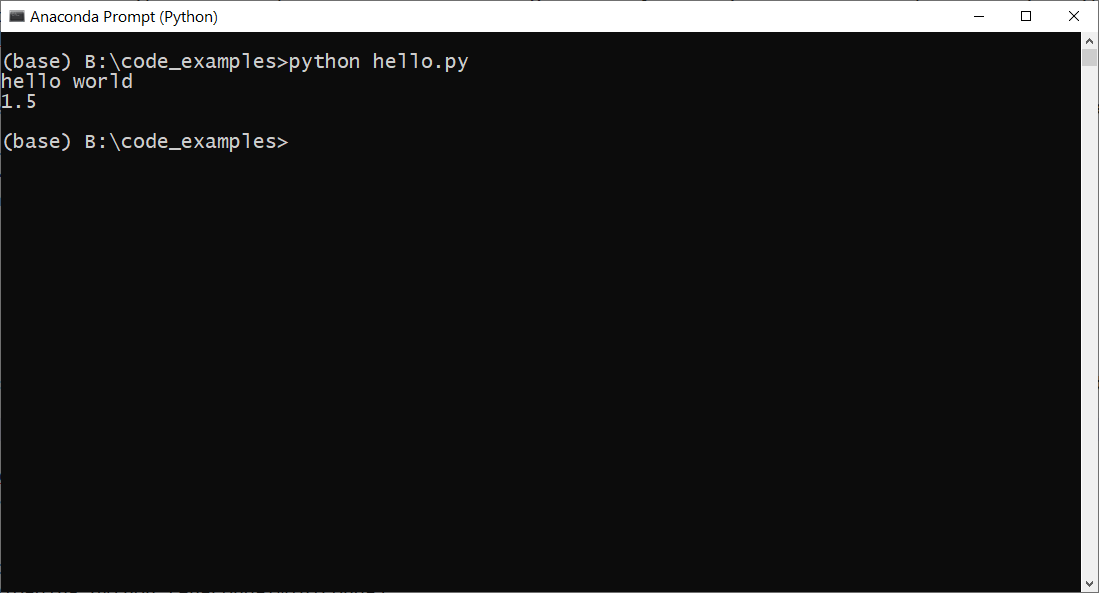
\includegraphics{screenshots/Ch01_04.PNG}

Certain scenarios will dictate whether you are writing code in an
interactive REPL session, or running code via scripts. Most of my work,
I debug initial code using the REPL, and then save the finalized code
and run the entire set of procedures through a script.

\section{Some Extra Notes}\label{some-extra-notes}

I use \href{https://notepad-plus-plus.org/}{Notepad++} to write much of
my code. Here is what the prior set of code looks like, showing
Notepad++ and the file itself:

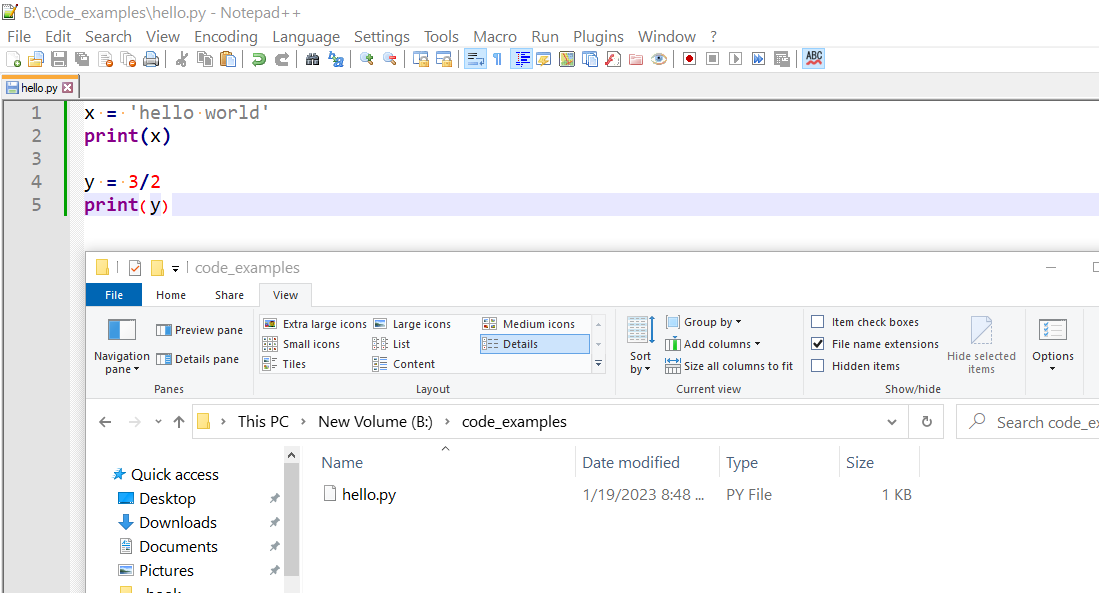
\includegraphics{screenshots/Ch01_05.PNG}

Notepad++ knows that a \texttt{.py} file is a python file, and so gives
nice code formatting. It also allows you to set an option to see
whitespace, which will become more important later when writing
conditional code blocks in python. (You should not write code in a
program that formats your text, such as Microsoft Word, as its
auto-formatting can cause errors in your code.)

But there are other options to help you write python code. On occasion
at my work I use Visual Studio (VS) Code, which is an entire IDE
(integrated development environment). This just means it has extra stuff
(like an embedded command prompt and github support). VS Code has
extensions for python as well as several other languages. Another
popular IDE for python is PyCharm. These again are mostly exchangeable,
I like Notepad++ for its simplicity.

\begin{tcolorbox}[enhanced jigsaw, toprule=.15mm, rightrule=.15mm, arc=.35mm, opacityback=0, coltitle=black, bottomrule=.15mm, left=2mm, opacitybacktitle=0.6, bottomtitle=1mm, colback=white, colframe=quarto-callout-note-color-frame, colbacktitle=quarto-callout-note-color!10!white, titlerule=0mm, breakable, title={Note}, toptitle=1mm, leftrule=.75mm]

Here are a few additional command line commands I use on a regular
basis:

\begin{itemize}
\tightlist
\item
  On Windows, to clear the terminal you can use \texttt{cls}, on
  Unix/MAC you can use \texttt{clear}
\item
  you can use \texttt{cat\ file.py} to print out the contents of a file
  to the terminal
\item
  you can use \texttt{mkdir} to make a new folder
\item
  you can pipe output to a file,
  e.g.~\texttt{python\ hello.py\ \textgreater{}\ log.txt} would save the
  output of the command above to the \texttt{log.txt} file instead of
  printing to the terminal.
\item
  if you use
  \texttt{python\ script.py\ \textgreater{}\textgreater{}\ log.txt} this
  \emph{appends} the output to log text file. Which is useful for
  repeated tasks that update over time.
\end{itemize}

\end{tcolorbox}

Another option to write python code (especially for individuals who do
scientific computing) is to use Jupyter Notebooks. Many beginner python
tutorials will suggest this. I will have a later chapter showing how to
make a standardized report using Jupyter Notebooks, but I do not suggest
this tool for beginners when first getting started. Many of the pieces
of information I will discuss in this book about project management are
difficult to control with Jupyter.

Now that you have the background to run python code, next chapter will
cover more of the basics of how to write python code.

\bookmarksetup{startatroot}

\chapter{Getting started writing python code}\label{sec-started}

\begin{tikzpicture}[overlay, remember picture]
\node[xshift=-1.5in,yshift=-1.5in] at (current page.north east) {
\includegraphics{chap_images/C02_latex.png}};
\end{tikzpicture}

While the prior chapter showed you how to run code, either in the REPL
or via scripts, this chapter will get you started writing python code
itself. The code examples shown via the text boxes I suggest typing into
a REPL session to follow along, but you could also save them into
\texttt{.py} scripts and run them directly as well. The grey portions
are what you would type into the terminal, and the blue boxes are what
should be printed out.

This chapter will walk through an introduction to working with numbers,
strings, booleans, lists, and dictionaries. These \emph{objects} are the
building blocks of pretty much all code in python.

\begin{tcolorbox}[enhanced jigsaw, toprule=.15mm, rightrule=.15mm, arc=.35mm, opacityback=0, coltitle=black, bottomrule=.15mm, left=2mm, opacitybacktitle=0.6, bottomtitle=1mm, colback=white, colframe=quarto-callout-note-color-frame, colbacktitle=quarto-callout-note-color!10!white, titlerule=0mm, breakable, title={Note}, toptitle=1mm, leftrule=.75mm]

On first read, this chapter (maybe all of them), will seem like a lot of
information, and will likely be boring. I suggest to follow along in the
REPL, but to \emph{skim} the chapters fairly fast (especially Chapters
2, 3 \& 4 on the basics of objects, strings, and looping). I have
intentionally tried to be fairly comprehensive for the basics. When
working on actual projects, you may need to revisit chapters to
understand and re-acquaint yourself with the topics. You do not become
an expert by reading a chapter one time, but by repeatedly writing code
for your own projects over time.

\end{tcolorbox}

\section{Numeric Values}\label{numeric-values}

To get started, you can think about python code as \emph{objects} and
\emph{operations} applied to those objects. So for example, if you run
the python code:

\begin{Shaded}
\begin{Highlighting}[]
\NormalTok{x }\OperatorTok{=} \DecValTok{1}
\NormalTok{y }\OperatorTok{=}\NormalTok{ x }\OperatorTok{+} \DecValTok{1}
\BuiltInTok{print}\NormalTok{(y)}
\end{Highlighting}
\end{Shaded}

\begin{verbatim}
2
\end{verbatim}

Here we first create an object, \texttt{x} that is \emph{assigned} a
value of 1 via the \texttt{=} symbol. We then create a second object,
\texttt{y}, that is assigned the value \texttt{x\ +\ 1}. And then
finally, we \texttt{print} the value of the \texttt{y} object.
\texttt{print} is a function, whose only purpose is to output the value
(or more specifically the string representation of that object), to the
terminal (or whatever location you tell python to output its results
to).

\begin{tcolorbox}[enhanced jigsaw, toprule=.15mm, rightrule=.15mm, arc=.35mm, opacityback=0, coltitle=black, bottomrule=.15mm, left=2mm, opacitybacktitle=0.6, bottomtitle=1mm, colback=white, colframe=quarto-callout-note-color-frame, colbacktitle=quarto-callout-note-color!10!white, titlerule=0mm, breakable, title={Note}, toptitle=1mm, leftrule=.75mm]

In the REPL, it is also possible to just type a single item on a line
and it will print the output to the terminal. So instead of
\texttt{print(y)}, in a REPL session you could just type \texttt{y} and
it will accomplish the same thing. In a script though, only
\texttt{print(y)} would send the output to the terminal.

\end{tcolorbox}

In the example above the objects were integer values. You can also have
float numeric objects as well. Python, unlike some programming
languages, does not force you to define the type of object before hand.

\begin{Shaded}
\begin{Highlighting}[]
\NormalTok{x }\OperatorTok{=} \OperatorTok{{-}}\DecValTok{1}
\NormalTok{y }\OperatorTok{=} \FloatTok{3.2}
\NormalTok{z }\OperatorTok{=}\NormalTok{ x}\OperatorTok{/}\NormalTok{y}
\BuiltInTok{print}\NormalTok{(z)}
\end{Highlighting}
\end{Shaded}

\begin{verbatim}
-0.3125
\end{verbatim}

When dealing with numeric values, python is smart and coerces \texttt{z}
here to be a float value, even though it uses one integer as input (even
with two integers, e.g.~\texttt{z\ =\ 1/2}, in python \texttt{z} will be
a float). You can see that here I did division, most of the math
operations are similar to what you would type into any calculator, with
the exception that powers use \texttt{**} instead of \texttt{\^{}}:

\begin{Shaded}
\begin{Highlighting}[]
\CommentTok{\# Showing off the different}
\CommentTok{\# math operations}
\NormalTok{x }\OperatorTok{=} \DecValTok{2}
\BuiltInTok{print}\NormalTok{(x }\OperatorTok{{-}} \DecValTok{1}\NormalTok{)}
\BuiltInTok{print}\NormalTok{(x }\OperatorTok{+} \DecValTok{1}\NormalTok{)}
\BuiltInTok{print}\NormalTok{(x}\OperatorTok{/}\DecValTok{2}\NormalTok{)}
\BuiltInTok{print}\NormalTok{(x}\OperatorTok{*}\DecValTok{2}\NormalTok{)}
\BuiltInTok{print}\NormalTok{(x}\OperatorTok{**}\DecValTok{3}\NormalTok{)      }\CommentTok{\# x to the third power}
\BuiltInTok{print}\NormalTok{(x}\OperatorTok{**}\NormalTok{(}\DecValTok{1}\OperatorTok{/}\DecValTok{2}\NormalTok{))  }\CommentTok{\# x to the 1/2 power (square root)}
\end{Highlighting}
\end{Shaded}

\begin{verbatim}
1
3
1.0
4
8
1.4142135623730951
\end{verbatim}

One special operator in python is to modify an objects numeric value. So
for example, to increment an objects value by one, you could do:

\begin{Shaded}
\begin{Highlighting}[]
\NormalTok{x }\OperatorTok{=} \DecValTok{1}
\NormalTok{x }\OperatorTok{=}\NormalTok{ x }\OperatorTok{+} \DecValTok{1}
\BuiltInTok{print}\NormalTok{(x)}
\end{Highlighting}
\end{Shaded}

\begin{verbatim}
2
\end{verbatim}

But it is easier to use the special notation of \texttt{x\ +=\ 1}:

\begin{Shaded}
\begin{Highlighting}[]
\NormalTok{x }\OperatorTok{=} \DecValTok{1}
\NormalTok{x }\OperatorTok{+=} \DecValTok{1}
\BuiltInTok{print}\NormalTok{(x)}
\end{Highlighting}
\end{Shaded}

\begin{verbatim}
2
\end{verbatim}

Note you can also do other mathematical operations, such as subtracting
\texttt{x\ -=\ 1}, multiplication \texttt{x\ *=\ 2}, division
\texttt{x\ /=\ 2}, or exponentiation \texttt{x\ **=\ 2}.

The final basic numeric examples to give are \texttt{//}, integer
division, and \texttt{\%}, the modulus operator. Integer division only
gives the whole numbers in a division problem, and modulus is the
remainder of the division problem.

\begin{Shaded}
\begin{Highlighting}[]
\NormalTok{x }\OperatorTok{=} \DecValTok{5}
\BuiltInTok{print}\NormalTok{(x}\OperatorTok{//}\DecValTok{2}\NormalTok{)}
\BuiltInTok{print}\NormalTok{(x }\OperatorTok{\%} \DecValTok{2}\NormalTok{)}
\end{Highlighting}
\end{Shaded}

\begin{verbatim}
2
1
\end{verbatim}

Later chapters discussing libraries intended to work with tabular data
(numpy and pandas), I will discuss numeric data processing in further
detail. As you often don't want to do math on a single object, but a
vector of multiple objects.

\section{Strings}\label{subsec-strings}

Another basic object you will often be using in python are strings. If
you enclose a set of characters inside of quotes, that results in a
string object. Here I even do addition of string objects, which
concatenates the two strings together.

\begin{Shaded}
\begin{Highlighting}[]
\NormalTok{x }\OperatorTok{=} \StringTok{"ABC"}
\NormalTok{y }\OperatorTok{=} \StringTok{"de"}
\NormalTok{z }\OperatorTok{=}\NormalTok{ x }\OperatorTok{+}\NormalTok{ y}
\BuiltInTok{print}\NormalTok{(z)}
\end{Highlighting}
\end{Shaded}

\begin{verbatim}
ABCde
\end{verbatim}

Strings can hold any alpha-numeric characters, so strings can hold text
representations of numbers. Note that adding two strings is not the same
as adding two numeric values! It concatenates the two strings together.

\begin{Shaded}
\begin{Highlighting}[]
\NormalTok{x }\OperatorTok{=} \StringTok{"1"}
\NormalTok{y }\OperatorTok{=} \StringTok{"3"}
\NormalTok{z }\OperatorTok{=}\NormalTok{ x }\OperatorTok{+}\NormalTok{ y}
\BuiltInTok{print}\NormalTok{(z)}
\end{Highlighting}
\end{Shaded}

\begin{verbatim}
13
\end{verbatim}

You can coerce strings to numeric values via the \texttt{int} and
\texttt{float} functions.

\begin{Shaded}
\begin{Highlighting}[]
\NormalTok{x }\OperatorTok{=} \StringTok{"1"}
\NormalTok{xi }\OperatorTok{=} \BuiltInTok{int}\NormalTok{(x)}
\NormalTok{xf }\OperatorTok{=} \BuiltInTok{float}\NormalTok{(x)}
\BuiltInTok{print}\NormalTok{(xi,}\StringTok{","}\NormalTok{,xf) }\CommentTok{\# can print multiple objects at once}
\end{Highlighting}
\end{Shaded}

\begin{verbatim}
1 , 1.0
\end{verbatim}

And vice-versa you can coerce numeric values to be strings via the
\texttt{str} function.

\begin{Shaded}
\begin{Highlighting}[]
\NormalTok{xi }\OperatorTok{=} \DecValTok{1}
\NormalTok{xf }\OperatorTok{=} \FloatTok{1.0} \CommentTok{\# if you use decimal, will be float}

\NormalTok{xsi }\OperatorTok{=} \BuiltInTok{str}\NormalTok{(xi)}
\NormalTok{xsf }\OperatorTok{=} \BuiltInTok{str}\NormalTok{(xf)}

\BuiltInTok{print}\NormalTok{(xsi }\OperatorTok{+} \StringTok{"|"} \OperatorTok{+}\NormalTok{ xsf) }\CommentTok{\#concat the strings}
\end{Highlighting}
\end{Shaded}

\begin{verbatim}
1|1.0
\end{verbatim}

\begin{tcolorbox}[enhanced jigsaw, toprule=.15mm, rightrule=.15mm, arc=.35mm, opacityback=0, coltitle=black, bottomrule=.15mm, left=2mm, opacitybacktitle=0.6, bottomtitle=1mm, colback=white, colframe=quarto-callout-note-color-frame, colbacktitle=quarto-callout-note-color!10!white, titlerule=0mm, breakable, title={Note}, toptitle=1mm, leftrule=.75mm]

I have introduced three functions so far, \texttt{print}, \texttt{int},
\texttt{float}, and \texttt{str}. Functions in python take the form
\texttt{function(input)}, so a particular name followed by two
parentheses.

\end{tcolorbox}

Strings can be enclosed either with single or double quotes. Note
however that special characters in strings can cause issues. Backward
slashes in windows path variables is one common example:

\begin{Shaded}
\begin{Highlighting}[]
\NormalTok{project\_path }\OperatorTok{=} \StringTok{"C:\textbackslash{}Project\textbackslash{}SubFolder"}
\NormalTok{project\_path }\CommentTok{\# Note no print statement}
\end{Highlighting}
\end{Shaded}

\begin{verbatim}
'C:\\Project\\SubFolder'
\end{verbatim}

\begin{tcolorbox}[enhanced jigsaw, toprule=.15mm, rightrule=.15mm, arc=.35mm, opacityback=0, coltitle=black, bottomrule=.15mm, left=2mm, opacitybacktitle=0.6, bottomtitle=1mm, colback=white, colframe=quarto-callout-note-color-frame, colbacktitle=quarto-callout-note-color!10!white, titlerule=0mm, breakable, title={Note}, toptitle=1mm, leftrule=.75mm]

What gets printed to the console is not necessarily the same text
representation of the object itself. For example, try
\texttt{x\ =\ "Line1\textbackslash{}nLine2"} and then type just
\texttt{x} at the terminal and see what is printed out, vs typing
\texttt{print(x)}. In this example, print interprets the line breaks in
the string, whereas just typing \texttt{x} in a REPL session does not.

\end{tcolorbox}

You can see that python inserted extra slashes! If you want the string
exactly as you typed it, you can use the \texttt{r""} string option,
which stands for \emph{real} string.

\begin{Shaded}
\begin{Highlighting}[]
\NormalTok{project\_path }\OperatorTok{=} \VerbatimStringTok{r"C:\textbackslash{}NoExtra\textbackslash{}BackSlashes"}
\BuiltInTok{print}\NormalTok{(project\_path)}
\end{Highlighting}
\end{Shaded}

\begin{verbatim}
C:\NoExtra\BackSlashes
\end{verbatim}

If you want a multi-line string in python, you can use triple quotes.
Note that this string has line breaks in the string object.

\begin{Shaded}
\begin{Highlighting}[]
\NormalTok{long\_note }\OperatorTok{=} \StringTok{\textquotesingle{}\textquotesingle{}\textquotesingle{}}
\StringTok{This is a long}
\StringTok{string note}
\StringTok{over multiple lines}
\StringTok{\textquotesingle{}\textquotesingle{}\textquotesingle{}}

\BuiltInTok{print}\NormalTok{(long\_note)}
\end{Highlighting}
\end{Shaded}

\begin{verbatim}

This is a long
string note
over multiple lines
\end{verbatim}

If you have a very long string, such as a url, that you don't want to
insert line breaks into, you can wrap the string in parenthesis. The
python interpreter just turns it into a string in the end:

\begin{Shaded}
\begin{Highlighting}[]
\NormalTok{long\_url }\OperatorTok{=}\NormalTok{ (}\StringTok{"Pretend I am a super "}
            \StringTok{"long url on a single line"}\NormalTok{)}

\BuiltInTok{print}\NormalTok{(long\_url)}
\end{Highlighting}
\end{Shaded}

\begin{verbatim}
Pretend I am a super long url on a single line
\end{verbatim}

I have an entire chapter, Chapter 3, devoted to more advanced usage of
strings.

\section{Booleans}\label{sec-bool}

Boolean objects can only have two values, \texttt{True} or
\texttt{False}.

\begin{Shaded}
\begin{Highlighting}[]
\BuiltInTok{print}\NormalTok{(}\DecValTok{1} \OperatorTok{==} \DecValTok{1}\NormalTok{)}
\BuiltInTok{print}\NormalTok{(}\DecValTok{2} \OperatorTok{==} \DecValTok{3}\NormalTok{)}
\end{Highlighting}
\end{Shaded}

\begin{verbatim}
True
False
\end{verbatim}

You can see I use \texttt{==} to do an equality comparison. Remember a
single \texttt{=} is for assignment. To use does not equal, the symbol
is \texttt{!=}:

\begin{Shaded}
\begin{Highlighting}[]
\BuiltInTok{print}\NormalTok{(}\StringTok{\textquotesingle{}a\textquotesingle{}} \OperatorTok{!=} \StringTok{\textquotesingle{}a\textquotesingle{}}\NormalTok{)}
\BuiltInTok{print}\NormalTok{(}\StringTok{\textquotesingle{}b\textquotesingle{}} \OperatorTok{!=} \StringTok{\textquotesingle{}c\textquotesingle{}}\NormalTok{)}
\end{Highlighting}
\end{Shaded}

\begin{verbatim}
False
True
\end{verbatim}

And then one can also use less than and greater than logic as well:

\begin{Shaded}
\begin{Highlighting}[]
\BuiltInTok{print}\NormalTok{(}\DecValTok{1} \OperatorTok{\textless{}} \DecValTok{1}\NormalTok{)}
\BuiltInTok{print}\NormalTok{(}\DecValTok{1} \OperatorTok{\textless{}=} \DecValTok{1}\NormalTok{)}
\BuiltInTok{print}\NormalTok{(}\DecValTok{2} \OperatorTok{\textgreater{}} \DecValTok{1}\NormalTok{)}
\BuiltInTok{print}\NormalTok{(}\DecValTok{2} \OperatorTok{\textgreater{}=} \DecValTok{1}\NormalTok{)}
\end{Highlighting}
\end{Shaded}

\begin{verbatim}
False
True
True
True
\end{verbatim}

Note one can also do less than checks with strings,
e.g.~\texttt{\textquotesingle{}a\textquotesingle{}\ \textless{}\ \textquotesingle{}b\textquotesingle{}}
is \texttt{True}, but I don't use this very frequently. The example
below shows a case that is probably not intended, as it accidentally
compares string representations of numbers instead of numbers directly.

\begin{Shaded}
\begin{Highlighting}[]
\BuiltInTok{print}\NormalTok{(}\StringTok{\textquotesingle{}10\textquotesingle{}} \OperatorTok{\textless{}} \StringTok{\textquotesingle{}2\textquotesingle{}}\NormalTok{)}
\end{Highlighting}
\end{Shaded}

\begin{verbatim}
True
\end{verbatim}

Often you use a boolean to do conditional logic in python code. So you
can have an \texttt{if} statement like below:

\begin{Shaded}
\begin{Highlighting}[]
\NormalTok{a }\OperatorTok{=} \DecValTok{1}

\ControlFlowTok{if}\NormalTok{ a }\OperatorTok{==} \DecValTok{1}\NormalTok{:}
  \BuiltInTok{print}\NormalTok{(a }\OperatorTok{+} \DecValTok{1}\NormalTok{)}
\end{Highlighting}
\end{Shaded}

\begin{verbatim}
2
\end{verbatim}

A special part of python syntax is that white space is special. To
denote that the \texttt{print} line is inside of the if statement, we
append several spaces to the front. The number of spaces does not
matter, it needs to be consistent though. (And you can technically also
use tabs instead of spaces, but I highly recommend against that, as it
can make editing the files a pain.)

Python uses \texttt{if}, \texttt{elif}, \texttt{else} for conditional
statements. Here is an if and an else example:

\begin{Shaded}
\begin{Highlighting}[]
\NormalTok{a }\OperatorTok{=} \DecValTok{1}

\ControlFlowTok{if}\NormalTok{ a }\OperatorTok{!=} \DecValTok{1}\NormalTok{:}
  \BuiltInTok{print}\NormalTok{(}\StringTok{\textquotesingle{}a does not equal 1\textquotesingle{}}\NormalTok{)}
  \BuiltInTok{print}\NormalTok{(a }\OperatorTok{+} \DecValTok{1}\NormalTok{)}
\ControlFlowTok{else}\NormalTok{:}
  \BuiltInTok{print}\NormalTok{(}\StringTok{\textquotesingle{}I am in the else part\textquotesingle{}}\NormalTok{)}
\end{Highlighting}
\end{Shaded}

\begin{verbatim}
I am in the else part
\end{verbatim}

The way these statements work, is that it checks if the first
\texttt{if} statement is true. If that statement is true, it executes
the code nested in the if part, \emph{and then exits the code block}. If
the \texttt{if} statement evaluates to False, it then executes the
\texttt{else} statement block for all other cases.

Sometimes you want to chain together multiple checks, e.g.~``if A, do Y,
else if B, do X''. To do that in python code, you would use \texttt{if}
and then \texttt{elif}.

\begin{Shaded}
\begin{Highlighting}[]
\NormalTok{a }\OperatorTok{=} \DecValTok{1}

\ControlFlowTok{if}\NormalTok{ a }\OperatorTok{!=} \DecValTok{1}\NormalTok{:}
  \BuiltInTok{print}\NormalTok{(}\StringTok{\textquotesingle{}a does not equal 1\textquotesingle{}}\NormalTok{)}
  \BuiltInTok{print}\NormalTok{(a }\OperatorTok{+} \DecValTok{1}\NormalTok{)}
\ControlFlowTok{elif}\NormalTok{ a }\OperatorTok{==} \DecValTok{1}\NormalTok{:}
  \BuiltInTok{print}\NormalTok{(}\StringTok{\textquotesingle{}I am in the elif part\textquotesingle{}}\NormalTok{)}
\ControlFlowTok{else}\NormalTok{:}
  \BuiltInTok{print}\NormalTok{(}\StringTok{\textquotesingle{}I am in the else part\textquotesingle{}}\NormalTok{)}
\end{Highlighting}
\end{Shaded}

\begin{verbatim}
I am in the elif part
\end{verbatim}

If an \texttt{elif} is true, it executes that block and then exits, same
as the \texttt{if} statement. So in the above code snippet, because the
\texttt{elif} statement is true, it never gets to the \texttt{else} part
of the conditional logic.

There is nothing that ties the different conditional statements
together, so not all sections need to reference the same item:

\begin{Shaded}
\begin{Highlighting}[]
\NormalTok{a }\OperatorTok{=} \DecValTok{1}
\NormalTok{b }\OperatorTok{=} \StringTok{\textquotesingle{}X\textquotesingle{}}

\ControlFlowTok{if}\NormalTok{ a }\OperatorTok{!=} \DecValTok{1}\NormalTok{:}
  \BuiltInTok{print}\NormalTok{(}\StringTok{\textquotesingle{}a does not equal 1\textquotesingle{}}\NormalTok{)}
\ControlFlowTok{elif}\NormalTok{ a }\OperatorTok{==} \DecValTok{2}\NormalTok{:}
  \BuiltInTok{print}\NormalTok{(}\StringTok{\textquotesingle{}a equals 2\textquotesingle{}}\NormalTok{)}
\ControlFlowTok{elif}\NormalTok{ b }\OperatorTok{==} \StringTok{\textquotesingle{}X\textquotesingle{}}\NormalTok{:}
  \BuiltInTok{print}\NormalTok{(}\StringTok{\textquotesingle{}I am in the b check elif part\textquotesingle{}}\NormalTok{)}
\ControlFlowTok{else}\NormalTok{:}
  \BuiltInTok{print}\NormalTok{(}\StringTok{\textquotesingle{}I am in the else part\textquotesingle{}}\NormalTok{)}
\end{Highlighting}
\end{Shaded}

\begin{verbatim}
I am in the b check elif part
\end{verbatim}

And you can write subsequent further conditional logic inside of a
conditional.

\begin{Shaded}
\begin{Highlighting}[]
\NormalTok{a }\OperatorTok{=} \DecValTok{1}
\NormalTok{b }\OperatorTok{=} \StringTok{\textquotesingle{}X\textquotesingle{}}

\ControlFlowTok{if}\NormalTok{ a }\OperatorTok{!=} \DecValTok{1}\NormalTok{:}
  \BuiltInTok{print}\NormalTok{(}\StringTok{\textquotesingle{}a does not equal 1\textquotesingle{}}\NormalTok{)}
  \ControlFlowTok{if}\NormalTok{ b }\OperatorTok{==} \StringTok{\textquotesingle{}X\textquotesingle{}}\NormalTok{:}
    \BuiltInTok{print}\NormalTok{(}\StringTok{\textquotesingle{}b check in first if\textquotesingle{}}\NormalTok{)}
\ControlFlowTok{else}\NormalTok{:}
  \BuiltInTok{print}\NormalTok{(}\StringTok{\textquotesingle{}I am in the else part\textquotesingle{}}\NormalTok{)}
  \ControlFlowTok{if}\NormalTok{ b }\OperatorTok{==} \StringTok{\textquotesingle{}X\textquotesingle{}}\NormalTok{:}
    \BuiltInTok{print}\NormalTok{(}\StringTok{\textquotesingle{}b check in elif\textquotesingle{}}\NormalTok{)}
\end{Highlighting}
\end{Shaded}

\begin{verbatim}
I am in the else part
b check in elif
\end{verbatim}

Sometimes in part of the condition, you want to do nothing. In those
cases, you can use \texttt{pass} inside the condition.

\begin{Shaded}
\begin{Highlighting}[]
\NormalTok{a }\OperatorTok{=} \DecValTok{1}

\ControlFlowTok{if}\NormalTok{ a }\OperatorTok{==} \DecValTok{1}\NormalTok{:}
  \ControlFlowTok{pass} \CommentTok{\# This snippet will print nothing}
\ControlFlowTok{else}\NormalTok{:}
  \BuiltInTok{print}\NormalTok{(}\StringTok{\textquotesingle{}I am in the else part\textquotesingle{}}\NormalTok{)}
\end{Highlighting}
\end{Shaded}

You typically want the more common conditions first in a series of if
statements, and less common conditions further down. So if the most
common condition you do nothing, and only in rarer conditions you
perform some action, this is a perfectly reasonable way to write your if
statements.

These examples compare just two objects, but you can compose multiple
conditional statements using \texttt{and} and \texttt{or}.

\begin{Shaded}
\begin{Highlighting}[]
\CommentTok{\# and example}
\NormalTok{a }\OperatorTok{=}\NormalTok{ (}\DecValTok{1} \OperatorTok{==} \DecValTok{1}\NormalTok{) }\KeywordTok{and}\NormalTok{ (}\DecValTok{2} \OperatorTok{==} \DecValTok{2}\NormalTok{)}
\BuiltInTok{print}\NormalTok{(a)}

\NormalTok{b }\OperatorTok{=}\NormalTok{ (}\DecValTok{1} \OperatorTok{==} \DecValTok{1}\NormalTok{) }\KeywordTok{and}\NormalTok{ (}\DecValTok{2} \OperatorTok{==} \DecValTok{3}\NormalTok{)}
\BuiltInTok{print}\NormalTok{(b)}

\CommentTok{\# or example}
\NormalTok{c }\OperatorTok{=}\NormalTok{ (}\DecValTok{1} \OperatorTok{==} \DecValTok{1}\NormalTok{) }\KeywordTok{or}\NormalTok{ (}\DecValTok{2} \OperatorTok{==} \DecValTok{3}\NormalTok{)}
\BuiltInTok{print}\NormalTok{(c)}
\end{Highlighting}
\end{Shaded}

\begin{verbatim}
True
False
True
\end{verbatim}

There are short hand operators though, ampersand for \texttt{and} and
the pipe for \texttt{or}:

\begin{Shaded}
\begin{Highlighting}[]
\CommentTok{\# ampersand for and}
\NormalTok{a }\OperatorTok{=}\NormalTok{ (}\DecValTok{1} \OperatorTok{==} \DecValTok{1}\NormalTok{) }\OperatorTok{\&}\NormalTok{ (}\DecValTok{2} \OperatorTok{==} \DecValTok{2}\NormalTok{)}
\BuiltInTok{print}\NormalTok{(a)}

\NormalTok{b }\OperatorTok{=}\NormalTok{ (}\DecValTok{1} \OperatorTok{==} \DecValTok{1}\NormalTok{) }\OperatorTok{\&}\NormalTok{ (}\DecValTok{2} \OperatorTok{==} \DecValTok{3}\NormalTok{)}
\BuiltInTok{print}\NormalTok{(b)}

\CommentTok{\# pipe for or}
\NormalTok{c }\OperatorTok{=}\NormalTok{ (}\DecValTok{1} \OperatorTok{==} \DecValTok{1}\NormalTok{) }\OperatorTok{|}\NormalTok{ (}\DecValTok{2} \OperatorTok{==} \DecValTok{3}\NormalTok{)}
\BuiltInTok{print}\NormalTok{(c)}
\end{Highlighting}
\end{Shaded}

\begin{verbatim}
True
False
True
\end{verbatim}

You technically don't need the parentheses in the above examples, but I
find it much easier to read the code that way and keep different terms
together:

\begin{Shaded}
\begin{Highlighting}[]
\CommentTok{\#       This is false        But this is true}
\NormalTok{a }\OperatorTok{=}\NormalTok{ ((}\DecValTok{1} \OperatorTok{==} \DecValTok{2}\NormalTok{) }\OperatorTok{\&}\NormalTok{ (}\DecValTok{2} \OperatorTok{==} \DecValTok{2}\NormalTok{)) }\OperatorTok{|}\NormalTok{ (}\DecValTok{4} \OperatorTok{==} \DecValTok{4}\NormalTok{)}
\BuiltInTok{print}\NormalTok{(a)}
\end{Highlighting}
\end{Shaded}

\begin{verbatim}
True
\end{verbatim}

But most of the time, if possible, I just break it down in code and make
the ultimate if statement line as simple as possible.

\begin{Shaded}
\begin{Highlighting}[]
\NormalTok{check1 }\OperatorTok{=}\NormalTok{ (}\DecValTok{1} \OperatorTok{==} \DecValTok{2}\NormalTok{) }\OperatorTok{\&}\NormalTok{ (}\DecValTok{2} \OperatorTok{==} \DecValTok{2}\NormalTok{) }\CommentTok{\# This is false}
\NormalTok{check2 }\OperatorTok{=}\NormalTok{ (}\DecValTok{4} \OperatorTok{==} \DecValTok{4}\NormalTok{)            }\CommentTok{\# This is true}

\ControlFlowTok{if}\NormalTok{ check1 }\OperatorTok{\&}\NormalTok{ check2:}
  \BuiltInTok{print}\NormalTok{(}\StringTok{\textquotesingle{}Both check1 and check2 are true\textquotesingle{}}\NormalTok{)}
\ControlFlowTok{elif}\NormalTok{ check1 }\OperatorTok{|}\NormalTok{ check2:}
  \BuiltInTok{print}\NormalTok{(}\StringTok{\textquotesingle{}At least one of check1 or check2 are true\textquotesingle{}}\NormalTok{)}
\ControlFlowTok{else}\NormalTok{:}
  \BuiltInTok{print}\NormalTok{(}\StringTok{\textquotesingle{}Neither check1 or check2 are true\textquotesingle{}}\NormalTok{)}
\end{Highlighting}
\end{Shaded}

\begin{verbatim}
At least one of check1 or check2 are true
\end{verbatim}

On occasion one does not use the math operators to generate the boolean
statements, but \texttt{is} or \texttt{is\ not}. Perhaps the most common
use of this is with the \texttt{None} object, what can be considered
missing data in python.

\begin{Shaded}
\begin{Highlighting}[]
\NormalTok{x }\OperatorTok{=} \VariableTok{None}

\ControlFlowTok{if}\NormalTok{ x }\KeywordTok{is} \VariableTok{None}\NormalTok{:}
  \BuiltInTok{print}\NormalTok{(}\StringTok{\textquotesingle{}x has no value\textquotesingle{}}\NormalTok{)}
\ControlFlowTok{else}\NormalTok{:}
  \BuiltInTok{print}\NormalTok{(}\StringTok{\textquotesingle{}x has some value\textquotesingle{}}\NormalTok{)}
\end{Highlighting}
\end{Shaded}

\begin{verbatim}
x has no value
\end{verbatim}

Technically when you write \texttt{a\ is\ b}, it not only checks the
objects values, but also that it references the \emph{exact same object}
in memory. Technically \texttt{x\ ==\ None} will work above, but it is
common practice to write it the \texttt{x\ is\ None} way. You can also
check the opposite condition via \texttt{is\ not\ None}:

\begin{Shaded}
\begin{Highlighting}[]
\NormalTok{x }\OperatorTok{=} \VariableTok{None}

\ControlFlowTok{if}\NormalTok{ x }\KeywordTok{is} \KeywordTok{not} \VariableTok{None}\NormalTok{:}
  \BuiltInTok{print}\NormalTok{(}\StringTok{\textquotesingle{}x has some value\textquotesingle{}}\NormalTok{)}
\ControlFlowTok{else}\NormalTok{:}
  \BuiltInTok{print}\NormalTok{(}\StringTok{\textquotesingle{}x is None\textquotesingle{}}\NormalTok{)}
\end{Highlighting}
\end{Shaded}

\begin{verbatim}
x is None
\end{verbatim}

For a final example, one can drop the comparison operators or if
statements entirely. If you pass an ``empty'' object to an if statement,
python checks to see if the object has any elements at all, and returns
\texttt{True} if it does. So if you pass in an empty string, the if
statement returns \texttt{False} here:

\begin{Shaded}
\begin{Highlighting}[]
\NormalTok{x }\OperatorTok{=} \StringTok{\textquotesingle{}\textquotesingle{}}

\ControlFlowTok{if}\NormalTok{ x:}
  \BuiltInTok{print}\NormalTok{(}\StringTok{\textquotesingle{}x has some value\textquotesingle{}}\NormalTok{)}
\ControlFlowTok{else}\NormalTok{:}
  \BuiltInTok{print}\NormalTok{(}\StringTok{\textquotesingle{}x is an empty string\textquotesingle{}}\NormalTok{)}
\end{Highlighting}
\end{Shaded}

\begin{verbatim}
x is an empty string
\end{verbatim}

This works for other python objects, such as empty lists and
dictionaries, which will be illustrated in the subsequent section.

\section{Lists}\label{lists}

It is important for beginners to have an understanding of different
objects that are containers for other objects. The first is a
\emph{list} object. A list contains multiple other objects, and you
create a list by placing items inside brackets, and separating the items
via commas. It is easier to show than to explain in words!

\begin{Shaded}
\begin{Highlighting}[]
\NormalTok{x }\OperatorTok{=}\NormalTok{ [}\DecValTok{1}\NormalTok{,}\DecValTok{2}\NormalTok{,}\DecValTok{3}\NormalTok{]}
\BuiltInTok{print}\NormalTok{(x)}
\end{Highlighting}
\end{Shaded}

\begin{verbatim}
[1, 2, 3]
\end{verbatim}

Lists can hold different object types, it can contain both strings and
numeric values in the same list for example. Here I also show that lists
can contain other defined python objects.

\begin{Shaded}
\begin{Highlighting}[]
\NormalTok{a }\OperatorTok{=} \DecValTok{1}
\NormalTok{b }\OperatorTok{=} \StringTok{\textquotesingle{}z\textquotesingle{}}
\NormalTok{x }\OperatorTok{=}\NormalTok{ [a,b,}\DecValTok{3}\NormalTok{]}
\BuiltInTok{print}\NormalTok{(x)}
\end{Highlighting}
\end{Shaded}

\begin{verbatim}
[1, 'z', 3]
\end{verbatim}

You can split items in a list onto multiple lines in the python
interpreter, it knows to look for the end bracket to know the input to
the list is finished. So the resulting list below is exactly the same as
\texttt{x\ =\ {[}1,2,3{]}}, just a different way to write it (it can be
nice to split very long lists onto multiple lines for readability in
your code).

\begin{Shaded}
\begin{Highlighting}[]
\CommentTok{\# it is ok to define lists}
\CommentTok{\# over multiple lines}
\NormalTok{x }\OperatorTok{=}\NormalTok{ [}\DecValTok{1}\NormalTok{,}
     \DecValTok{2}\NormalTok{,}
     \DecValTok{3}\NormalTok{]}

\CommentTok{\# it is the same as earlier}
\CommentTok{\# on a single line}
\BuiltInTok{print}\NormalTok{(x)}
\end{Highlighting}
\end{Shaded}

\begin{verbatim}
[1, 2, 3]
\end{verbatim}

A common error when working with lists is to forget the comma. With
numeric values this will often result in an error, but with strings it
can sometimes not result in an error, since python will just implicitly
concatenate the strings together. For an example:

\begin{Shaded}
\begin{Highlighting}[]
\CommentTok{\# This is probably not what was intended}
\NormalTok{x }\OperatorTok{=}\NormalTok{ [}\StringTok{\textquotesingle{}a\textquotesingle{}} \StringTok{\textquotesingle{}b\textquotesingle{}}\NormalTok{, }\StringTok{\textquotesingle{}c\textquotesingle{}}\NormalTok{]}
\BuiltInTok{print}\NormalTok{(x)}
\end{Highlighting}
\end{Shaded}

\begin{verbatim}
['ab', 'c']
\end{verbatim}

So here the comma between the first two strings was omitted, so the
resulting list is just two elements, with the first being
\texttt{\textquotesingle{}ab\textquotesingle{}}.

\begin{tcolorbox}[enhanced jigsaw, toprule=.15mm, rightrule=.15mm, arc=.35mm, opacityback=0, coltitle=black, bottomrule=.15mm, left=2mm, opacitybacktitle=0.6, bottomtitle=1mm, colback=white, colframe=quarto-callout-note-color-frame, colbacktitle=quarto-callout-note-color!10!white, titlerule=0mm, breakable, title={Note}, toptitle=1mm, leftrule=.75mm]

One benefit to writing lists on multiple lines, is you can use
\emph{column} editing in various text editors. In Notepad++, you can
hold down the alt key and select multiple rows to edit at once. Most
advanced text editors have a similar feature.

\end{tcolorbox}

You can access individual items in a list via its index. Note in python
that list indices start at 0, not at 1, so the first element of a list
will be 0, the second element will be 1, etc.

\begin{Shaded}
\begin{Highlighting}[]
\NormalTok{y }\OperatorTok{=}\NormalTok{ [}\StringTok{\textquotesingle{}a\textquotesingle{}}\NormalTok{,}\StringTok{\textquotesingle{}b\textquotesingle{}}\NormalTok{,}\StringTok{\textquotesingle{}c\textquotesingle{}}\NormalTok{]}
\BuiltInTok{print}\NormalTok{(y[}\DecValTok{0}\NormalTok{])}
\BuiltInTok{print}\NormalTok{(y[}\DecValTok{1}\NormalTok{])}
\BuiltInTok{print}\NormalTok{(y[}\DecValTok{2}\NormalTok{])}
\end{Highlighting}
\end{Shaded}

\begin{verbatim}
a
b
c
\end{verbatim}

You can also use \emph{negative} indices to access items in reverse
order in a list. So -1 accesses the last item in a list, -2 the second
to last item, etc.

\begin{Shaded}
\begin{Highlighting}[]
\NormalTok{y }\OperatorTok{=}\NormalTok{ [}\StringTok{\textquotesingle{}a\textquotesingle{}}\NormalTok{,}\StringTok{\textquotesingle{}b\textquotesingle{}}\NormalTok{,}\StringTok{\textquotesingle{}c\textquotesingle{}}\NormalTok{]}
\BuiltInTok{print}\NormalTok{(y[}\OperatorTok{{-}}\DecValTok{1}\NormalTok{])}
\BuiltInTok{print}\NormalTok{(y[}\OperatorTok{{-}}\DecValTok{2}\NormalTok{])}
\end{Highlighting}
\end{Shaded}

\begin{verbatim}
c
b
\end{verbatim}

Finally in terms of accessing multiple items in a list, you can use
slice notation. So \texttt{x{[}1:3{]}} would access the 2nd and 3rd
items in the list (it is equivalent to \texttt{{[},)} notation is
mathematics, so the left end of the slice is closed, and the right end
of the slice is open.

\begin{Shaded}
\begin{Highlighting}[]
\NormalTok{y }\OperatorTok{=}\NormalTok{ [}\StringTok{\textquotesingle{}a\textquotesingle{}}\NormalTok{,}\StringTok{\textquotesingle{}b\textquotesingle{}}\NormalTok{,}\StringTok{\textquotesingle{}c\textquotesingle{}}\NormalTok{]}
\BuiltInTok{print}\NormalTok{(y[}\DecValTok{1}\NormalTok{:}\DecValTok{3}\NormalTok{]) }\CommentTok{\# note it returns a list!}
\end{Highlighting}
\end{Shaded}

\begin{verbatim}
['b', 'c']
\end{verbatim}

You can also use \texttt{x{[}1:{]}} to indicate, ``give me the 2nd item
in the list until the end'', or \texttt{x{[}:3{]}} to ``give me the
first 3 items in the list.

One can create an empty list, simply by assigning \texttt{{[}{]}} to a
value. Another useful trick to know is that you can do a boolean check
for an empty list.

\begin{Shaded}
\begin{Highlighting}[]
\NormalTok{x }\OperatorTok{=}\NormalTok{ []}

\ControlFlowTok{if}\NormalTok{ x:}
  \BuiltInTok{print}\NormalTok{(}\StringTok{\textquotesingle{}The x list is not empty\textquotesingle{}}\NormalTok{)}
\ControlFlowTok{else}\NormalTok{:}
  \BuiltInTok{print}\NormalTok{(}\StringTok{\textquotesingle{}x is empty\textquotesingle{}}\NormalTok{)}
\end{Highlighting}
\end{Shaded}

\begin{verbatim}
x is empty
\end{verbatim}

An empty list has no objects, so if you try to access an object it will
return an error. Above if you try to use \texttt{x{[}0{]}}, you will get
an error \texttt{index\ out\ of\ range}.

Another boolean operation on lists is to check if an element is
contained in that list.

\begin{Shaded}
\begin{Highlighting}[]
\NormalTok{x }\OperatorTok{=}\NormalTok{ [}\StringTok{\textquotesingle{}a\textquotesingle{}}\NormalTok{,}\StringTok{\textquotesingle{}b\textquotesingle{}}\NormalTok{,}\StringTok{\textquotesingle{}c\textquotesingle{}}\NormalTok{]}

\ControlFlowTok{if} \StringTok{\textquotesingle{}d\textquotesingle{}} \KeywordTok{in}\NormalTok{ x:}
  \BuiltInTok{print}\NormalTok{(}\StringTok{\textquotesingle{}The list has a d element\textquotesingle{}}\NormalTok{)}
\ControlFlowTok{elif} \StringTok{\textquotesingle{}c\textquotesingle{}} \KeywordTok{in}\NormalTok{ x:}
  \BuiltInTok{print}\NormalTok{(}\StringTok{\textquotesingle{}The list has a c element\textquotesingle{}}\NormalTok{)}
\ControlFlowTok{else}\NormalTok{:}
  \BuiltInTok{print}\NormalTok{(}\StringTok{\textquotesingle{}x has neither d or c\textquotesingle{}}\NormalTok{)}
\end{Highlighting}
\end{Shaded}

\begin{verbatim}
The list has a c element
\end{verbatim}

One special piece of information you need to know about lists is that
they are \emph{mutable}. What does that mean exactly? It means that we
can modify the contents of a list. So for example, we can replace a
single item in a list.

\begin{Shaded}
\begin{Highlighting}[]
\NormalTok{y }\OperatorTok{=}\NormalTok{ [}\StringTok{\textquotesingle{}a\textquotesingle{}}\NormalTok{,}\StringTok{\textquotesingle{}b\textquotesingle{}}\NormalTok{,}\StringTok{\textquotesingle{}c\textquotesingle{}}\NormalTok{]}
\BuiltInTok{print}\NormalTok{(y)}

\NormalTok{y[}\DecValTok{1}\NormalTok{] }\OperatorTok{=} \StringTok{\textquotesingle{}Z\textquotesingle{}}
\BuiltInTok{print}\NormalTok{(y)}
\end{Highlighting}
\end{Shaded}

\begin{verbatim}
['a', 'b', 'c']
['a', 'Z', 'c']
\end{verbatim}

For a more complicated example, lists can point to other lists. Because
lists are mutable, you can modify the inner list here, and the outer
list reflects this change.

\begin{Shaded}
\begin{Highlighting}[]
\NormalTok{x }\OperatorTok{=}\NormalTok{ [}\StringTok{\textquotesingle{}a\textquotesingle{}}\NormalTok{,}\StringTok{\textquotesingle{}b\textquotesingle{}}\NormalTok{,}\StringTok{\textquotesingle{}c\textquotesingle{}}\NormalTok{]}
\NormalTok{y }\OperatorTok{=}\NormalTok{ [}\DecValTok{1}\NormalTok{, x]}
\BuiltInTok{print}\NormalTok{(y)}

\CommentTok{\# if we alter x}
\CommentTok{\# y points to }
\CommentTok{\# the altered x list}
\NormalTok{x[}\DecValTok{1}\NormalTok{] }\OperatorTok{=} \StringTok{\textquotesingle{}Z\textquotesingle{}}
\BuiltInTok{print}\NormalTok{(y)}
\end{Highlighting}
\end{Shaded}

\begin{verbatim}
[1, ['a', 'b', 'c']]
[1, ['a', 'Z', 'c']]
\end{verbatim}

The way to think about this, the list \texttt{y} here does not actually
contain the contents of \texttt{x}, it simply \emph{points to} the
\texttt{x} object. So if the \texttt{x} object gets changed, it points
to that new \texttt{x} object.

This may seem quite in the weeds, but it is an important feature of the
python programming language. It allows one to write many different
algorithms in a simpler fashion when one can alter lists in place.

You can concatenate two lists together by adding them:

\begin{Shaded}
\begin{Highlighting}[]
\NormalTok{x }\OperatorTok{=}\NormalTok{ [}\StringTok{\textquotesingle{}a\textquotesingle{}}\NormalTok{,}\StringTok{\textquotesingle{}b\textquotesingle{}}\NormalTok{,}\StringTok{\textquotesingle{}c\textquotesingle{}}\NormalTok{]}
\NormalTok{y }\OperatorTok{=}\NormalTok{ [}\DecValTok{1}\NormalTok{,}\DecValTok{2}\NormalTok{]}
\NormalTok{z }\OperatorTok{=}\NormalTok{ x }\OperatorTok{+}\NormalTok{ y}
\BuiltInTok{print}\NormalTok{(z)}
\end{Highlighting}
\end{Shaded}

\begin{verbatim}
['a', 'b', 'c', 1, 2]
\end{verbatim}

You can also make a repeated list via multiplication:

\begin{Shaded}
\begin{Highlighting}[]
\NormalTok{x }\OperatorTok{=}\NormalTok{ [}\StringTok{\textquotesingle{}a\textquotesingle{}}\NormalTok{,}\StringTok{\textquotesingle{}b\textquotesingle{}}\NormalTok{,}\StringTok{\textquotesingle{}c\textquotesingle{}}\NormalTok{]}
\NormalTok{y }\OperatorTok{=}\NormalTok{ [}\DecValTok{1}\NormalTok{]}
\BuiltInTok{print}\NormalTok{(y}\OperatorTok{*}\DecValTok{3} \OperatorTok{+}\NormalTok{ x}\OperatorTok{*}\DecValTok{2}\NormalTok{)}
\end{Highlighting}
\end{Shaded}

\begin{verbatim}
[1, 1, 1, 'a', 'b', 'c', 'a', 'b', 'c']
\end{verbatim}

Lists have several \emph{methods} to modify their contents; two commons
one used are sorting and reversing:

\begin{Shaded}
\begin{Highlighting}[]
\NormalTok{x }\OperatorTok{=}\NormalTok{ [}\DecValTok{3}\NormalTok{,}\DecValTok{1}\NormalTok{,}\DecValTok{2}\NormalTok{]}

\NormalTok{x.sort() }\CommentTok{\# sorting the list}
\BuiltInTok{print}\NormalTok{(x)}

\NormalTok{x.reverse() }\CommentTok{\# reverse ordering}
\BuiltInTok{print}\NormalTok{(x)}
\end{Highlighting}
\end{Shaded}

\begin{verbatim}
[1, 2, 3]
[3, 2, 1]
\end{verbatim}

\begin{tcolorbox}[enhanced jigsaw, toprule=.15mm, rightrule=.15mm, arc=.35mm, opacityback=0, coltitle=black, bottomrule=.15mm, left=2mm, opacitybacktitle=0.6, bottomtitle=1mm, colback=white, colframe=quarto-callout-note-color-frame, colbacktitle=quarto-callout-note-color!10!white, titlerule=0mm, breakable, title={Note}, toptitle=1mm, leftrule=.75mm]

When you sort or reverse a list, it does this operation and modifies the
list \emph{in-place}. So the code \texttt{y\ =\ x.sort()} is probably
incorrect, as \texttt{x.sort()} returns nothing. So \texttt{y} does not
equal the sorted list, but is \texttt{None}.

\end{tcolorbox}

Methods are special functions that are tied to particular objects. So
look like \texttt{object.method(input)}. They will always be demarcated
from the base object by a period -- so this means you cannot use a
period in a variable name. For example if you type \texttt{q.i\ =\ 1}
into the terminal it will return an error that
\texttt{q\ is\ not\ defined}. These methods can take additional
arguments (they are just like functions), but these examples just use
the default. For example, you can sort in descending order:

\begin{Shaded}
\begin{Highlighting}[]
\NormalTok{x }\OperatorTok{=}\NormalTok{ [}\DecValTok{3}\NormalTok{,}\DecValTok{1}\NormalTok{,}\DecValTok{2}\NormalTok{]}

\NormalTok{x.sort(reverse}\OperatorTok{=}\VariableTok{True}\NormalTok{) }\CommentTok{\# passing arg}
\BuiltInTok{print}\NormalTok{(x)}
\end{Highlighting}
\end{Shaded}

\begin{verbatim}
[3, 2, 1]
\end{verbatim}

\begin{tcolorbox}[enhanced jigsaw, toprule=.15mm, rightrule=.15mm, arc=.35mm, opacityback=0, coltitle=black, bottomrule=.15mm, left=2mm, opacitybacktitle=0.6, bottomtitle=1mm, colback=white, colframe=quarto-callout-note-color-frame, colbacktitle=quarto-callout-note-color!10!white, titlerule=0mm, breakable, title={Note}, toptitle=1mm, leftrule=.75mm]

This is the first example I have shown for a function that has a
\emph{keyword} argument, so instead of \texttt{function(input)} it is
\texttt{function(keyword=input)}. Functions can take multiple arguments,
such as \texttt{function(input1,input2)}. In this scenario the order of
the arguments matter, and you may use keyword arguments to distinguish
between the inputs. I will go into more details on this in a subsequent
chapter on defining your own functions.

\end{tcolorbox}

You can also append or remove items from lists:

\begin{Shaded}
\begin{Highlighting}[]
\NormalTok{x }\OperatorTok{=}\NormalTok{ [}\DecValTok{3}\NormalTok{,}\DecValTok{1}\NormalTok{,}\DecValTok{2}\NormalTok{]}

\NormalTok{x.append(}\StringTok{\textquotesingle{}a\textquotesingle{}}\NormalTok{) }\CommentTok{\# appending an item to end of list}
\BuiltInTok{print}\NormalTok{(x)}

\NormalTok{x.remove(}\DecValTok{1}\NormalTok{) }\CommentTok{\# removing an item}
\BuiltInTok{print}\NormalTok{(x)}
\end{Highlighting}
\end{Shaded}

\begin{verbatim}
[3, 1, 2, 'a']
[3, 2, 'a']
\end{verbatim}

To find the specific location of an item in a list, you can use the
index method:

\begin{Shaded}
\begin{Highlighting}[]
\NormalTok{x }\OperatorTok{=}\NormalTok{ [}\StringTok{\textquotesingle{}a\textquotesingle{}}\NormalTok{,}\StringTok{\textquotesingle{}b\textquotesingle{}}\NormalTok{,}\StringTok{\textquotesingle{}c\textquotesingle{}}\NormalTok{]}

\CommentTok{\# will be 1, the 2nd item in a list}
\NormalTok{bindex }\OperatorTok{=}\NormalTok{ x.index(}\StringTok{\textquotesingle{}b\textquotesingle{}}\NormalTok{)}
\BuiltInTok{print}\NormalTok{(bindex)}
\end{Highlighting}
\end{Shaded}

\begin{verbatim}
1
\end{verbatim}

There are other methods to lists I have not shown here, if you run the
\texttt{dir} command on an object, it will print out all of its
potential methods. I encourage you to experiment yourself and see how
the other methods, like \texttt{count} or \texttt{pop}, work.

\begin{Shaded}
\begin{Highlighting}[]
\NormalTok{x }\OperatorTok{=}\NormalTok{ [}\StringTok{\textquotesingle{}a\textquotesingle{}}\NormalTok{,}\StringTok{\textquotesingle{}b\textquotesingle{}}\NormalTok{,}\StringTok{\textquotesingle{}c\textquotesingle{}}\NormalTok{]}

\CommentTok{\# you can look at the methods}
\CommentTok{\# for a object using dir(object)}
\NormalTok{me }\OperatorTok{=} \BuiltInTok{dir}\NormalTok{(x)}

\CommentTok{\# there are many more! only}
\CommentTok{\# printing a few to save space}
\BuiltInTok{print}\NormalTok{(me[}\OperatorTok{{-}}\DecValTok{6}\NormalTok{:])}
\end{Highlighting}
\end{Shaded}

\begin{verbatim}
['index', 'insert', 'pop', 'remove', 'reverse', 'sort']
\end{verbatim}

Sometimes you want a list like object, but you do not want it to be
mutable (so you cannot do operations like change a single value, append,
or sort the list). This may occur if you have a set of constants in your
script, and you know they should never be altered. Placing them in a
\emph{tuple} is one way to ensure they don't accidentally get modified.
Tuple's look mostly the same as a list, but use parentheses instead of
square brackets:

\begin{Shaded}
\begin{Highlighting}[]
\NormalTok{y }\OperatorTok{=}\NormalTok{ (}\DecValTok{1}\NormalTok{,}\DecValTok{2}\NormalTok{,}\DecValTok{3}\NormalTok{)}
\NormalTok{y[}\DecValTok{1}\NormalTok{] }\OperatorTok{=} \DecValTok{5} \CommentTok{\# this will give an error}
\end{Highlighting}
\end{Shaded}

\begin{verbatim}
TypeError: 'tuple' object does not support item assignment
\end{verbatim}

You can convert a list to a tuple via the \texttt{tuple} command:

\begin{Shaded}
\begin{Highlighting}[]
\NormalTok{y }\OperatorTok{=}\NormalTok{ [}\DecValTok{1}\NormalTok{,}\DecValTok{2}\NormalTok{,}\DecValTok{3}\NormalTok{]}
\NormalTok{z }\OperatorTok{=} \BuiltInTok{tuple}\NormalTok{(y)}
\NormalTok{y[}\DecValTok{1}\NormalTok{] }\OperatorTok{=} \DecValTok{5} \CommentTok{\# this is ok}
\BuiltInTok{print}\NormalTok{(y) }\CommentTok{\# can see y list is updated}
\NormalTok{z[}\DecValTok{1}\NormalTok{] }\OperatorTok{=} \DecValTok{5} \CommentTok{\# this is not, again cannot modify tuple}
\end{Highlighting}
\end{Shaded}

\begin{verbatim}
[1, 5, 3]
\end{verbatim}

\begin{verbatim}
TypeError: 'tuple' object does not support item assignment
\end{verbatim}

Or vice versa convert a tuple to a list via the \texttt{list} command:

\begin{Shaded}
\begin{Highlighting}[]
\NormalTok{z }\OperatorTok{=}\NormalTok{ (}\DecValTok{1}\NormalTok{,}\DecValTok{2}\NormalTok{,}\DecValTok{3}\NormalTok{)}
\NormalTok{y }\OperatorTok{=} \BuiltInTok{list}\NormalTok{(z)}
\NormalTok{y[}\DecValTok{1}\NormalTok{] }\OperatorTok{=} \DecValTok{5} \CommentTok{\# this is ok}
\BuiltInTok{print}\NormalTok{(y)}
\NormalTok{z[}\DecValTok{1}\NormalTok{] }\OperatorTok{=} \DecValTok{5} \CommentTok{\# this is not, again cannot modify tuple}
\end{Highlighting}
\end{Shaded}

\begin{verbatim}
[1, 5, 3]
\end{verbatim}

\begin{verbatim}
TypeError: 'tuple' object does not support item assignment
\end{verbatim}

One last note about tuples, you can assign multiple objects at the same
time. So you can do:

\begin{Shaded}
\begin{Highlighting}[]
\NormalTok{x, y }\OperatorTok{=} \DecValTok{1}\NormalTok{, }\DecValTok{2}
\BuiltInTok{print}\NormalTok{(x,y)}
\end{Highlighting}
\end{Shaded}

\begin{verbatim}
1 2
\end{verbatim}

This is called \emph{tuple unpacking}. The reason it is called this is
that when you \emph{don't} unpack the multiple values separated by a
comma, it returns a tuple.

\begin{Shaded}
\begin{Highlighting}[]
\NormalTok{t }\OperatorTok{=} \DecValTok{1}\NormalTok{, }\DecValTok{2}
\BuiltInTok{print}\NormalTok{(t)}
\end{Highlighting}
\end{Shaded}

\begin{verbatim}
(1, 2)
\end{verbatim}

And you can assign more than two values:

\begin{Shaded}
\begin{Highlighting}[]
\NormalTok{a,b,c,d }\OperatorTok{=}\NormalTok{ (}\DecValTok{1}\NormalTok{,}\StringTok{\textquotesingle{}a\textquotesingle{}}\NormalTok{,}\DecValTok{6}\NormalTok{,}\OperatorTok{{-}}\FloatTok{1.2}\NormalTok{)}
\BuiltInTok{print}\NormalTok{(a,b,c,d)}
\end{Highlighting}
\end{Shaded}

\begin{verbatim}
1 a 6 -1.2
\end{verbatim}

This can be convenient in various for loop examples (shown in Chapter
4), and when functions return multiple values (shown in Chapter 5).
Besides this though, tuples are not as commonly used as lists in my
experience. But one example use they have is illustrated in the next
section, where one has a need to use immutable tuples for dictionaries.

\section{Dictionaries}\label{dictionaries}

The second major container of items in python is a dictionary. So to
access items in a list, it is just a set order, the first element is
\texttt{mylist{[}0{]}}, the second element is \texttt{mylist{[}1{]}},
etc. Sometimes you want to be able to access the elements by simpler
names, e.g.~imagine you had a list to contain a persons information:

\begin{Shaded}
\begin{Highlighting}[]
\CommentTok{\# using a list to hold data}
\NormalTok{x }\OperatorTok{=}\NormalTok{ [}\StringTok{\textquotesingle{}Andy Wheeler\textquotesingle{}}\NormalTok{,}\StringTok{\textquotesingle{}Data Scientist\textquotesingle{}}\NormalTok{,}\StringTok{\textquotesingle{}2019\textquotesingle{}}\NormalTok{]}
\end{Highlighting}
\end{Shaded}

To access the name item, you need to know it is in the 0 index, the
title item is in the 1 index, etc. It is probably easier to refer to
this data via a dictionary.

\begin{Shaded}
\begin{Highlighting}[]
\CommentTok{\# using a list to hold data}
\NormalTok{d }\OperatorTok{=}\NormalTok{ \{}\StringTok{\textquotesingle{}name\textquotesingle{}}\NormalTok{: }\StringTok{\textquotesingle{}Andy Wheeler\textquotesingle{}}\NormalTok{,}
     \StringTok{\textquotesingle{}title\textquotesingle{}}\NormalTok{:}\StringTok{\textquotesingle{}Data Scientist\textquotesingle{}}\NormalTok{,}
     \StringTok{\textquotesingle{}start\_year\textquotesingle{}}\NormalTok{: }\DecValTok{2019}\NormalTok{\}}

\BuiltInTok{print}\NormalTok{(d)}
\end{Highlighting}
\end{Shaded}

\begin{verbatim}
{'name': 'Andy Wheeler', 'title': 'Data Scientist', 'start_year':
2019}
\end{verbatim}

Now, it is easier to access an individual item via
\texttt{dict{[}key{]}}, so if I only want the name, I just reference
that explicitly:

\begin{Shaded}
\begin{Highlighting}[]
\CommentTok{\# Grabbing the specific name element}
\BuiltInTok{print}\NormalTok{(d[}\StringTok{\textquotesingle{}name\textquotesingle{}}\NormalTok{])}
\end{Highlighting}
\end{Shaded}

\begin{verbatim}
Andy Wheeler
\end{verbatim}

The terminology for dictionaries is that they have \emph{keys} that
reference \emph{values}. Values can be anything: numeric values,
strings, lists, other dictionaries, etc. Keys however need to be
\emph{immutable}, even though dictionaries themselves are mutable (so
you cannot use a list as a key, but you can use a tuple). Here we can
modify the values of the original \texttt{d} dictionary I created. You
can also add in a new element once the dictionary is created.

\begin{Shaded}
\begin{Highlighting}[]
\CommentTok{\# Modifying the start\_year element}
\NormalTok{d[}\StringTok{\textquotesingle{}start\_year\textquotesingle{}}\NormalTok{] }\OperatorTok{=} \DecValTok{2020}

\CommentTok{\# Adding in a new element tenure}
\NormalTok{d[}\StringTok{\textquotesingle{}tenure\textquotesingle{}}\NormalTok{] }\OperatorTok{=} \DecValTok{3}

\BuiltInTok{print}\NormalTok{(d[}\StringTok{\textquotesingle{}name\textquotesingle{}}\NormalTok{])}
\BuiltInTok{print}\NormalTok{(d[}\StringTok{\textquotesingle{}title\textquotesingle{}}\NormalTok{])}
\BuiltInTok{print}\NormalTok{(d[}\StringTok{\textquotesingle{}start\_year\textquotesingle{}}\NormalTok{])}
\BuiltInTok{print}\NormalTok{(d[}\StringTok{\textquotesingle{}tenure\textquotesingle{}}\NormalTok{])}
\end{Highlighting}
\end{Shaded}

\begin{verbatim}
Andy Wheeler
Data Scientist
2020
3
\end{verbatim}

Most often people use strings for keys, since the main benefit of
dictionaries over lists is to have a name for referencing specific
objects. But it can be a number as well. So say you had numeric ids in
another database referencing specific locations, it may make sense to
write your dictionary using those same numeric identifiers.

\begin{Shaded}
\begin{Highlighting}[]
\CommentTok{\# You can have numeric values}
\CommentTok{\# as a dictionary key}
\NormalTok{d }\OperatorTok{=}\NormalTok{ \{\} }\CommentTok{\# can init a dict as empty}
\NormalTok{d[}\DecValTok{101}\NormalTok{] }\OperatorTok{=}\NormalTok{ \{}\StringTok{\textquotesingle{}address\textquotesingle{}}\NormalTok{: }\StringTok{\textquotesingle{}Penny Lane\textquotesingle{}}\NormalTok{, }\StringTok{\textquotesingle{}tot\_crimes\textquotesingle{}}\NormalTok{: }\DecValTok{1}\NormalTok{\}}
\NormalTok{d[}\DecValTok{202}\NormalTok{] }\OperatorTok{=}\NormalTok{ \{}\StringTok{\textquotesingle{}address\textquotesingle{}}\NormalTok{: }\StringTok{\textquotesingle{}Outer Space\textquotesingle{}}\NormalTok{, }\StringTok{\textquotesingle{}tot\_crimes\textquotesingle{}}\NormalTok{: }\DecValTok{42}\NormalTok{\}}

\CommentTok{\# These show a dictionary inside of a dictionary}
\BuiltInTok{print}\NormalTok{(d[}\DecValTok{101}\NormalTok{])}
\BuiltInTok{print}\NormalTok{(d[}\DecValTok{202}\NormalTok{])}
\end{Highlighting}
\end{Shaded}

\begin{verbatim}
{'address': 'Penny Lane', 'tot_crimes': 1}
{'address': 'Outer Space', 'tot_crimes': 42}
\end{verbatim}

And similar to empty lists, an empty dictionary will return
\texttt{False} in a boolean if statement:

\begin{Shaded}
\begin{Highlighting}[]
\NormalTok{d }\OperatorTok{=}\NormalTok{ \{\} }\CommentTok{\# can init a dict as empty}

\ControlFlowTok{if}\NormalTok{ d:}
  \BuiltInTok{print}\NormalTok{(}\StringTok{\textquotesingle{}The dictionary d is not empty\textquotesingle{}}\NormalTok{)}
\ControlFlowTok{else}\NormalTok{:}
  \BuiltInTok{print}\NormalTok{(}\StringTok{\textquotesingle{}The dictionary d is empty\textquotesingle{}}\NormalTok{)}
\end{Highlighting}
\end{Shaded}

\begin{verbatim}
The dictionary d is empty
\end{verbatim}

There are \emph{many} types of more complicated objects in python, the
very first example in the preface showed an example working with
\emph{datetime} objects. But under the hood, they are often just a
container to conduct different operations on the objects I listed above:
numeric values, strings, lists, and dictionaries.


\backmatter

\end{document}
